\chapter{Game Design}
\label{chap:game_design}

\section{Obiettivo}
\label{obiettivo}

L’obiettivo del lavoro di Tesi è stato quello di portare un pubblico che non conosce la tematica, ma è abituato a determinati contesti, che dimostra un interesse, anche non spiccato, verso questo bagaglio culturale, a mostrare curiosità nei confronti del tema del pre-Cinema.

Il pubblico a cui si fa riferimento è quello di ragazzi tra gli 11 ed i 18 anni, frequentanti perciò la scuola media inferiore e superiore. Con lo sviluppo, negli ultimi decenni, di differenti tipologie di media e di canali di informazione, tale fascia di età risulta estremamente abituata a contesti ludici o altre definizioni di intrattenimento sviluppate in forma digitale.
Ogni scelta di design è stata perciò effettuata tenendo conto del pubblico fruitore del prodotto finale, cercando perciò di limitare l’uso di metafore di gioco, o meccaniche che potessero risultare troppo complesse per un pubblico giovane.
Nonostante i ragazzi in tale fascia di età abbiano mostrato familiarità con il mezzo videoludico, abbiamo notato varie capacità di approccio per quanto riguarda l’input e l’interfacciamento con il prodotto sviluppato. Abbiamo quindi ritenuto opportuno tener conto anche delle differenti abilità di gioco ed abitudini ad utilizzare differenti dispositivi di input, e di conseguenza a prendere delle scelte di design che fossero state coerenti con quest’aspetto.

Risulta importante specificare che l’obiettivo primario del lavoro non è stato quello di insegnare o inculcare concetti ai ragazzi fruitori del gioco. Un approccio del genere avrebbe portato il prodotto ad essere caratterizzato da una forma didascalica e didattica, che avrebbe rischiato di sortire persino l’effetto opposto nei confronti degli utenti del gioco, l’essere noioso e poco divertente, poco appetibile ad un pubblico giovane.
Si è data perciò particolare importanza alla scelta di meccaniche di gioco divertenti, ambientazioni che avessero generato curiosità e stupore ed un gameplay stimolante. Elementi accompagnati dalla possibilità di fruire di schede informative e contenuti inerenti la tematica che si è deciso di affrontare.

\subsection{Piattaforma di riferimento e momenti museali}
\label{sec:piattaforma_di_riferimento}

Una scelta cruciale nella produzione di una qualsiasi forma di videogioco, è quella relativa alle piattaforme per cui sviluppare il prodotto finale. Risulta evidente come tale scelta influenzi pesantemente ogni elemento di design, dalla caratterizzazione più o meno dettagliata delle ambientazioni all’interfacciamento dell’utente.

Una prima analisi è stata quella relativa ai momenti museali a cui poter far riferimento. Per momenti museali intendiamo gli intervalli temporali in relazione all’entrata del pubblico in museo:
\begin{itemize}
	\item \textbf{Pre-visita.} Sono quei momenti in cui il pubblico si incuriosisce riguardo l’ambito museale e si interessa di una possibile visita. Volantini, passaparola, pubblicità, sono elementi che influenzano e caratterizzano il momento della pre-visita.
	\item \textbf{Visita.}  È l’intervallo temporale che il pubblico trascorre all’interno del museo, viene caratterizzato perciò dai contenuti veri e propri, oltre che da tutti gli altri elementi presenti all’interno del museo.
	\item \textbf{Post-visita.} Sono i momenti successivi alla visita del museo. Sono direttamente correlati alla soddisfazione provata dal pubblico, che può consigliare la visita ad altre persone, oltre che svolgere attività coerenti al contesto museale e provare interesse nei confronti di ciò che ha visitato.
\end{itemize}
Si è innanzitutto valutata la possibilità di sviluppare un prodotto fruibile all’interno del museo. L’applicazione avrebbe perciò avuto lo scopo di accompagnare la visita, tramite dei piccoli giochi, che avrebbero permesso di osservare alcuni degli elementi, presenti all’interno del museo, da prospettive diverse, generando nel pubblico una maggiore curiosità riguardo argomenti che sarebbero potuti risultare noiosi o poco interessanti. Un prodotto con un simile approccio è naturalmente sviluppabile per dispositivi mobili.

Secondo una nostra ipotesi, avvalorata anche da una personale ricerca di mercato, applicazioni del genere risultano molto interessanti per fasce di età inferiori rispetto a quella di riferimento per il progetto di Tesi.
I bambini, infatti, risultano particolarmente attratti da applicazioni semplici, immediate e veloci che possono rendere più piacevole la visita al museo, anche in compagnia di amici.
Ci si è quindi concentrati nei due restanti momenti museali, quelli precedenti e successivi alla visita.

Risulta importante specificare che la scelta della piattaforma di riferimento è stata effettuata anche in base alle meccaniche di gioco che si sono delineate durante le fasi di design del gameplay.
Abbiamo valutato la possibilità di sviluppare un casual game per dispositivi mobili, ma tale scelta avrebbe portato ad un prodotto superficiale, che sarebbe potuto risultare troppo semplicistico per il tema da voler affrontare.

\begin{figure}%[h]
	\centering
	% left bottom right top
	%\includegraphics[clip= true, width= 0.8\columnwidth, trim= 1.5cm 3.0cm 0.6cm 0.0cm]{images/gameDesign/01_megarun.jpg}
	\includegraphics[width= 0.8\columnwidth]{images/gameDesign/01_megarun.jpg}
	\caption{Megarun: esempio di casual game.}
	\label{fig:casual_game}
\end{figure}

La natura \textit{platform/puzzle} ideata durante le fasi di Design, ci ha spinto a sviluppare il prodotto per PC e console. Tali piattaforme permettono l’utilizzo di dispositivi di input più adatti alle tipologie di \textit{gameplay} che sono state progettate, oltre che fornire una qualità visiva più consona all’estetica con cui si vuole caratterizzare il prodotto finito.
Tale scelta fornisce una ampia libertà di design, permettendo di sviluppare meccaniche complesse e profonde \textit{storyline}, tipiche di una produzione di buon livello.

Concludendo, si è quindi scelto di sviluppare il videogioco per PC e console, con lo scopo di generare curiosità riguardo l’ambito del pre-cinema, attraverso meccaniche di gioco mirate, ambientazioni caratteristiche e schede informative studiate per fornire un buon supporto. Questo approccio risulta quindi coerente con i momenti museali di pre e post-visita, generando interesse nei confronti di un tema non ancora approfondito, o fornendo un buon metodo per osservare tematiche già note, apprese da una precedente visita, da un differente punto di vista.

\section{Meccaniche}
\label{sec:meccaniche}

Le meccaniche di gioco sono forse il nucleo più importante di una produzione videoludica di qualità, sono gli elementi che rimangono quando estetica, tecnologia e storia vengono meno, ed anche in queste condizioni, il prodotto, se caratterizzato da buone meccaniche, deve risultare piacevole ed efficace.
Il gameplay deve essere caratterizzato da regole semplici, ma allo stesso tempo flessibili, devono essere facili da capire, ma difficili da padroneggiare.

Il concetto di meccanica di gioco è strettamente legato a quello delle regole del game design, argomento che quindi non si limita ai videogiochi, ma a tutte le forme di intrattenimento che fanno riferimento al termine astratto di \textit{gioco}.
Abbiamo quindi fatto particolare attenzione al fornire al giocatore uno spazio di gioco in cui le meccaniche fornite avessero assicurato una sensazione di libertà, regolata però da limiti per circoscriverne le possibilità.
Il prodotto deve essere caratterizzato da pochi elementi di gameplay, ma che permettano al giocatore, entro certi limiti, di sentirsi libero di agire.

Ogni meccanica deve quindi essere semplice da capire e da utilizzare, ma deve richiedere un impegno ed uno studio progressivo per essere padroneggiata al meglio ed essere sfruttata in tutte le sue potenzialità.

Questo concetto è bene espresso nel libro \textit{The Art Of Game Design} \cite{artOfGameDesign}:
“Molti game designers sono d’accordo sul fatto che azioni interessanti che emergono col tempo siano la caratteristica di un buon gioco. Di conseguenza, il rapporto tra azioni significative e azioni di base è una buona misura di quanto un gioco emerga col tempo. Un gioco risulta elegante se permette al giocatore un piccolo numero di azioni di base, ma un grande numero di azioni significative.”

Chiaramente si tratta di un discorso soggettivo, ma ciò su cui abbiamo molto lavorato è stato trovare meccaniche di gioco semplici, ma che avessero permesso un vasto numero di possibilità in termini di \textit{level design} e possibilità del giocatore.

\subsection{Elementi Platform}
\label{platform}
Il videogioco sviluppato presenta molte caratteristiche tipiche della categoria dei \textit{platform}.
Abbiamo scelto di utilizzare alcune meccaniche platform perché, oltre ad essere coerente con la rappresentazione che abbiamo deciso di creare durante le fasi di \textit{brainstorming}, è un genere che sta tornando ad occupare una importante fetta di mercato. 

Il genere dei platform è nato nei primi anni ’80, ed ha avuto nel tempo una diffusione grandissima. Secondo wikipedia \cite{platform_wikipedia} , nel 1998 occupava il 15\% del mercato, nel 2006 ha avuto il suo massimo calo, arrivando ad occupare solo il 2\%, ma dal 2010 ha avuto una rinnovata popolarità, dovuta anche alla grande varietà degli \textit{endless runner} che sono esplosi soprattutto nel mondo mobile. Anche la fervente attività degli sviluppatori indipendenti, sviluppatasi negli ultimi anni, ha fatto sì che il genere acquisisse di nuovo importanza nel settore. Tali studi, potendo contare su budget e mezzi limitati, hanno trovato, nel genere, un’importante base su cui poter costruire.

Per quanto riguarda il puro lato estetico, come mostrato in Figura~\ref{fig:platform_proportions}, il personaggio principale ha proporzioni non realistiche, molto accentuate in larghezza piuttosto che in altezza, con una proporzione che si avvicina all'1:1.

\begin{figure}%[h]
	\centering
	% left bottom right top
	%\includegraphics[clip= true, width= 0.8\columnwidth, trim= 1.5cm 3.0cm 0.6cm 0.0cm]{images/gameDesign/01_megarun.jpg}
	\includegraphics[width= 0.9\columnwidth]{images/gameDesign/02_braid_SM.jpg}
	\caption{Proporzione del personaggio di un platform game: Braid e SuperMario.}
	\label{fig:platform_proportions}
\end{figure}

Caratteristici dei platform sono quegli elementi di gioco che richiedono soprattutto delle abilità di reazione e concentrazione del giocatore, come corsa, salto o usare piattaforme.

Per quanto riguarda il movimento del personaggio, abbiamo deciso di ricorrere ad una corsa bidirezionale, a velocità uniforme in entrambe le direzioni ed indipendente dalla pressione del tasto di riferimento o dell’inclinazione della levetta analogica del controller. Questo assicura un padroneggiamento più veloce della meccanica, che, per le caratteristiche di gioco, non richiede una eccessiva complessità.
La velocità massima di corsa è raggiunta in maniera non esattamente istantanea, questo per assicurarsi un movimento non troppo brusco e quindi poco intuitivo.

La bidirezionalità fa sì che il personaggio si giri nel caso venga indicato un movimento opposto rispetto all’attuale direzione. Questo permette di raggiungere di nuovo, dove permesso dal design dei livelli, posti già visitati in precedenza (Figura~\ref{fig:platform_corsa}). Tale scelta non deve essere presa in maniera superficiale, in quanto ci si deve assicurare che elementi di gioco, incontrati in differenti momenti della partita, non si interfaccino in maniera problematica tra di loro. 
\begin{figure}%[h]
	\centering
	\includegraphics[width= \columnwidth]{images/gameDesign/03.jpg}
	\caption{Movimenti di corsa nel prototipo sviluppato}
	\label{fig:platform_corsa}
\end{figure}
In \textit{SuperMario Bros.} (Capitolo~\ref{sec:stato_arte_super_mario}) il personaggio può cambiare direzione, ma la camera non può tornare indietro, quindi, quando il personaggio arriva al bordo sinistro, è come se sbatta contro un muro invisibile.
La tipologia di gioco definita \textit{Endless Runner} invece, evita il problema impedendo al giocatore di invertire la direzione, nella maggior parte dei casi imponendo una corsa indipendente dall’input del giocatore o in altri casi semplicemente rallentabile o accelerabile (Figura~\ref{fig:platform_corsa_reali}).

\begin{figure}%[h]
	\centering
	\includegraphics[width= \columnwidth]{images/gameDesign/04.jpg}
	\caption{Esempi di corsa: SuperMario e JetpackJoyride.}
	\label{fig:platform_corsa_reali}
\end{figure}

Per il salto, abbiamo deciso inizialmente di assegnare al personaggio una forza fissa verso l’alto, in seguito alla pressione del relativo bottone. Alcuni videogiochi invece assegnano una forza dipendente in maniera proporzionale dalla pressione del giocatore. Sono chiaramente due approcci differenti, il secondo fa sì che il salto sia una meccanica più complessa da padroneggiare, ma assicura delle possibilità di gameplay in più.
Durante i testing effettuati, abbiamo notato delle frequenti difficoltà nell’effettuare i salti, possiamo perciò pensare di prendere provvedimenti in tal senso, magari dando al giocatore un maggior controllo sulla potenza di salto, o limitando le sezioni in cui l’utilizzo del salto risulti troppo cruciale.

I movimenti del personaggio in aria sono controllabili attraverso i tasti direzionali. Perciò, dopo il salto o in seguito ad una caduta, il giocatore può direzionare o aggiustare la traiettoria di discesa. Non tutti i videogiochi platform assicurano tale comportamento, ma abbiamo ritenuto potesse essere utile per non frustrare eccessivamente il giocatore in seguito ad un salto non perfettamente calibrato al momento dello stacco.
La caduta del personaggio è soggetta ad una gravità 3 volte superiore al normale, è un elemento già presente in \textit{SuperMario} e ampiamente utilizzato nei giochi del genere per garantire una sensazione di repentinità al giocatore. La velocità di caduta è comunque limitata per garantirne il controllo.

\begin{figure}%[h]
	\centering
	\includegraphics[width= 0.8\columnwidth]{images/gameDesign/05.jpg}
	\caption{Personaggio del prototipo, durante un salto.}
	\label{fig:platform_salto}
\end{figure}

Oltre alle meccaniche di corsa e salto, abbiamo dato la possibilità al personaggio di salire e scendere le scale. Questa è una meccanica non essenziale, che non aggiunge possibilità rispetto a quelle che non possa garantire una serie di salti, ma garantisce una maggiore sensazione di libertà al giocatore e permette una migliore pulizia per quanto riguarda il \textit{level design}. Le scale infatti, come mostrato in Figura~\ref{fig:platform_scala_piattaforme}, consentono di raggiungere luoghi per cui, altrimenti sarebbero state necessarie numerose piattaforme, che avrebbero potuto rendere la realizzazione dei livelli molto difficoltosa e confusa.

\begin{figure}%[h]
	\centering
	\includegraphics[width= 0.8\columnwidth]{images/gameDesign/06.jpg}
	\caption{Confronto tra utilizzo di scale e piattaforme equivalenti.}
	\label{fig:platform_scala_piattaforme}
\end{figure}

Le meccaniche di salto, controllo del personaggio in aria ed utilizzo scale sono state ispirate dal videogioco \textit{Braid} (Capitolo~\ref{sec:stato_arte_braid}), anche qui infatti il salto fornisce una forza indipendente dalla pressione del tasto e la possibilità di controllare il personaggio in caduta è una meccanica importante di gioco, anche se, rispetto a \textit{Braid}, la forza impressa dal salto risulta meno forte e la gravità in caduta più espressiva, i movimenti in \textit{Braid} appaiono più naturali, nel nostro caso invece più repentini ed eccessivi.

Sono state incluse nel gioco anche delle piattaforme mobili (Figura~\ref{fig:platform_piattaforme_mobili}). Queste hanno un movimento lineare tra due punti, uno dei quali raggiungibile dal personaggio, mentre l’altro si pone come obiettivo finale del movimento. Sono un elemento che mette alla prova le abilità di tempismo e di concentrazione del giocatore. Tali piattaforme risultano attraversabili dal basso verso l’alto, questo per permettere una maggiore libertà di approccio all’utente.
Durante i test effettuati, abbiamo notato che, spesso, i giocatori fanno fatica a comprendere i momenti esatti in cui la piattaforma cambia di direzione. Si sta perciò valutando se, nel prodotto finale non possa essere utile introdurre degli elementi che, graficamente, rappresentino dei limiti di inizio e fine corsa.

\begin{figure}%[h]
	\centering
	\includegraphics[width= 0.6\columnwidth]{images/gameDesign/07.jpg}
	\caption{Esempio di piattaforme mobili sviluppate.}
	\label{fig:platform_piattaforme_mobili}
\end{figure}

Graficamente, abbiamo deciso di rappresentare il terreno normale con una colorazione verde. Tale elemento non è attraversabile in nessuna direzione. Il personaggio collide sempre con esso.

Le piattaforme mobili vengono invece rappresentate con una colorazione blu scura, come si può osservare in Figura~\ref{fig:platform_piattaforme_mobili}.

Un altro terreno, che abbiamo deciso di sviluppare, permette di essere attraversato in entrambe le direzioni, ma solo se il personaggio sta utilizzando una scala. Permette appunto di attraversare terreni normalmente non attraversabili, ma caratterizzati dalla presenza della scala. La colorazione per questo tipo di terreno rimane comunque quella verde. Abbiamo verificato, tramite test e prototipazione, che questa scelta non influisce sulla comprensibilità della meccanica, in quanto caratterizzata dalla presenza della scala.

Parallelamente abbiamo ritenuto necessario sviluppare una tipologia differente di terreno, che permette di essere superato dal basso, ad esempio con un salto del personaggio. Non è attraversabile dall’alto. Tale scelta apre la strada ad una nuova meccanica, in quanto realizza una via a “senso unico” che può essere utile in fase di \textit{level design}. Questo terreno invece, è differenziato dal resto tramite una colorazione blu più tenue rispetto alle piattaforme mobili.

Le 3 tipologie di terreno possono essere osservate in Figura~\ref{fig:platform_terreni}.

\begin{figure}%[h]
	\centering
	\includegraphics[width= \columnwidth]{images/gameDesign/08.jpg}
	\caption{Esempi delle tre tipologie di terreno sviluppate.}
	\label{fig:platform_terreni}
\end{figure}

\subsection{Elementi Puzzle}
\label{elementi_puzzle}

Oltre alle meccaniche \textit{Platform}, che richiedono soprattutto reattività, tempismo e concentrazione del giocatore, il videogioco presenta anche caratteristiche tipiche del genere dei \textit{Puzzle Games}.

Questa categoria di videogiochi enfatizza soprattutto la risoluzione di enigmi e puzzles. Il giocatore deve perciò possedere le capacità di osservare la situazione in cui si trova il personaggio, analizzarne gli elementi, e capire in che modo debbano essere sfruttati ed usati per superare una determinata sezione o raggiungere un obiettivo.
Sono perciò richieste quelle che il libro \textit{The Art Of Game Design}\cite{artOfGameDesign} definisce come abilità mentali (\textit{Mental Skills}), viene proposta di seguito una traduzione della sezione:
“Le abilità mentali includono le capacità di memoria, osservazione e risoluzione di puzzle. Sebbene alcune persone evitino giochi che richiedono troppo impegno per quanto riguarda queste capacità, è raro che i giochi non le includano anche in piccola parte, perché i giochi sono interessanti quando ci sono decisioni interessanti da prendere, e prendere decisioni è una abilità mentale.”

Risulta necessario specificare che, nella fase di \textit{Level Design}, abbiamo fatto particolare attenzione nel mescolare intelligentemente elementi \textit{platform} e \textit{puzzle}, in modo da essere in sintonia tra loro, senza che uno dei due elementi apparisse predominante sull’altro e che l’esperienza non risultasse eccessivamente frenetica e frustrante da un lato o lenta e noiosa dall’altro.
Le dinamiche puzzle ci hanno permesso anche di fare design riguardo il possibile utilizzo di strumenti particolari del pre-Cinema in maniera originale e curiosa (Capitolo~\ref{sec:meccaniche_precinema}), inserendo quindi elementi di gioco non presenti in altri esponenti del settore.
Elementi classici del puzzle game, che abbiamo inserito sono, ad esempio, leve, pulsanti, casse, porte, bilance e sequenze di bottoni.

Le leve (Figura~\ref{fig:platform_leve}) sono utilizzate per avere un effetto diretto sullo scenario di gioco. Generalmente, le abbiamo utilizzate per spostare elementi dell’ambientazione o attivare meccanismi.

\begin{figure}%[h]
	\centering
	\includegraphics[width= \columnwidth]{images/gameDesign/09.jpg}
	\caption{Esempio di leva. Utilizzata per interagire con un elemento dello scenario.}
	\label{fig:platform_leve}
\end{figure}

I pulsanti a pressione possono essere intesi, concettualmente, come le leve, hanno un effetto immediato su alcuni elementi dello scenario. Nel nostro caso in particolare, abbiamo preferito associarli ad aperture e chiusure di porte, portoni o elementi traslabili che impediscono o permettono il passaggio del personaggio da una zona all’altra di gioco. Questa scelta è stata fatta per permettere al giocatore di capire immediatamente l’effetto di un bottone, spesso anche prima di premerlo.

L’attivazione dei bottoni avviene nel momento in cui il personaggio sale su di essi, hanno perciò un funzionamento a pressione. L’effetto diretto avviene al momento dell’attivazione. Quando il personaggio scende, i bottoni possono disattivarsi e quindi invertire l’effetto sortito sullo scenario di gioco o rimanere attivi e mantenerlo nel tempo. Tale scelta dipende dal particolare utilizzo e quindi da scelte di \textit{level design}.

I bottoni, come già specificato, vengono attivati dalla pressione su di essi, sia che venga applicata dal personaggio principale, che da un nemico (Capitolo~\ref{sec:nemici}). Come mostrato in Figura~\ref{fig:platform_bottoni} abbiamo comunque ritenuto utile inserire delle casse come elemento di gioco. Esse permettono di premere i bottoni senza la presenza del personaggio, oltre che salirci sopra per raggiungere posti più elevati.

\begin{figure}%[h]
	\centering
	\includegraphics[width= \columnwidth]{images/gameDesign/10.jpg}
	\caption{Bottoni premuti dal personaggio e da una cassa.}
	\label{fig:platform_bottoni}
\end{figure}

Coerentemente con il concetto di pressione e pesi, abbiamo introdotto nel gioco anche delle bilance (Figura~\ref{fig:platform_bilancia}). Per semplicità, abbiamo ipotizzato che ogni elemento di gioco abbia una massa, relativamente alla bilancia, di una unità. Ipotizzando perciò che in un piatto ci sia una cassa, per avere una situazione di equilibro, è sufficiente che sull’altro piatto ci sia il personaggio. La bilancia, come le leve, permette di attivare un elemento dello scenario. È stata utilizzata, ad esempio, per un enigma in cui è necessario spostare un numero di nemici sufficienti in un piatto, per far sì che l’altro si alzi e attivi un bottone.

\begin{figure}%[h]
	\centering
	\includegraphics[width= 0.5\columnwidth]{images/gameDesign/11.jpg}
	\caption{Bilancia.}
	\label{fig:platform_bilancia}
\end{figure}

Un altro elemento interessante sono le sequenze di bottoni (Figura~\ref{fig:platform_sequenza_bottoni}). Queste hanno lo stesso funzionamento dei bottoni singoli ma, per interagire con una porta è necessario attivarli tutti nella giusta sequenza. Se il primo bottone premuto è quello giusto, questo rimane attivo, se il secondo non è giusto, vengono disattivati tutti e la sequenza deve ricominciare dall’inizio. Quando vengono premuti tutti i bottoni nella giusta sequenza, viene attivato l’elemento dello scenario prestabilito, nel nostro caso le sequenze di bottoni sono sempre state utilizzate per aprire porte.

\begin{figure}%[h]
	\centering
	\includegraphics[width= 0.7\columnwidth]{images/gameDesign/12.jpg}
	\caption{Sequenza di bottoni.}
	\label{fig:platform_sequenza_bottoni}
\end{figure}

Viene riportata di seguito l’analisi di un enigma presente in uno dei livelli sviluppati. Nella Figura~\ref{fig:platform_enigma} si possono notare alcuni elementi non ancora analizzati, come il nemico, la lanterna magica o la stella, fare riferimento ai Capitolo~\ref{sec:nemici}, \ref{sec:meccaniche_precinema} e \ref{sec:elementi_rigiocabilita} per approfondimenti più dettagliati sul loro utilizzo, che qui verrà spiegato in maniera superficiale.

\begin{figure}%[h]
	\centering
	\includegraphics[width= \columnwidth]{images/gameDesign/13.jpg}
	\caption{Esempio di enigma.}
	\label{fig:platform_enigma}
\end{figure}

Come spesso avviene nei vari livelli sviluppati, la via per proseguire non richiede la completa risoluzione dell’enigma, ma solo la parte più semplice di esso, così da permettere, anche ai giocatori non interessati al raccoglimento di tutti i collezionabili, di proseguire con la partita.
In figura~\ref{fig:platform_enigma} vengono contrassegnati con la stessa lettera i bottoni e le relative porte che vengono azionate.

Il personaggio può subito porsi sopra il bottone “e” e notare l’apertura della relativa porta, che conduce ad una stanza con un altro bottone. Il giocatore capisce che la pressione di questo bottone è l’unico modo per proseguire. Raggiunge perciò un luogo favorevole per piazzare a terra la lanterna magica e sfruttarne il vento prodotto per spingere la cassa, bloccata però dalla porta “e”. Il personaggio deve quindi tornare sul bottone “e” e permettere alla cassa di premere il bottone “f”. Il personaggio può quindi raggiungere le scale e salire. Il nemico, premendo il pulsante “g”, attiva una porta con degli spuntoni, che blocca il raggiungimento dell’uscita, posta nella zona in alto a destra dell’immagine. Si deve perciò fare attenzione ad avere il giusto tempismo.

Come si può notare dall’immagine, il personaggio principale può quindi raggiungere l’uscita, ma rimane una stella da raccogliere. Come già specificato, solo la parte obbligatoria dell’enigma è stata risolta, ma non quella opzionale per il raccoglimento della stella.

Il giocatore può quindi, una volta salita la scala ed arrivati sul livello del nemico, scendere dalla scala, aspettare che il nemico si volti verso la porta/macigno, saltare il nemico, premere il bottone “b” e permettere così al nemico di cadere al piano inferiore. Questo, camminando, raggiungerà la zona con il bottone “e”, senza la possibilità di uscirne. Continuerà perciò ad attivare la porta che conduce alla stanza con la stella, che potrà quindi essere agilmente raccolta dal personaggio. Una volta collezionata, si può proseguire lungo il livello.
La seconda immagine in Figura~\ref{fig:platform_enigma} mostra l’enigma completamente risolto.

\subsection{Camera e Puntatore}
\label{sec:camera_e_puntatore}

Per quando riguarda la camera, abbiamo fatto in modo che questa fosse sempre approssimativamente centrata sul personaggio principale. In realtà usa una funzione che ne ammorbidisce il movimento, non segue perciò perfettamente il personaggio, ma tende in breve tempo alla sua posizione. Questa scelta è stata presa per rendere l’effetto meno brusco e quindi più gradevole alla vista.
Abbiamo anche ritenuto necessario includere la possibilità di evitare che la camera inquadri porzioni di scena non previste. È stata perciò valutata la capacità di gestire dei limiti della scena. Questa opzione è stata utilizzata solamente nel livello centrale, che funge da accesso agli altri livelli, ma sicuramente può fornire un mezzo ulteriore, in fase di design di altre meccaniche.

In seguito al design della meccanica di gioco principale, quella della Lanterna Magica (Capitolo~\ref{sec:meccaniche_precinema}), si è valutata la possibilità di inserire, per non confondere eccessivamente il giocatore, la possibilità di utilizzare un puntatore anche nelle normali fasi di gioco.

\begin{figure}%[h]
	\centering
	\includegraphics[width= 0.85\columnwidth]{images/gameDesign/15.jpg}
	\caption{Spostamento della camera in relazione alla posizione del personaggio e del puntatore.}
	\label{fig:camera_posizione_1_4}
\end{figure}

Il puntatore permette all’utente di spostare la camera dal personaggio principale ed osservare quindi porzioni di gioco che, normalmente, non sarebbero presenti nella visuale standard.
Il design del puntatore è stato un passaggio particolarmente difficile, che abbiamo perfezionato col tempo, in seguito allo sviluppo e test di vari prototipi.
Una delle prime versioni che abbiamo sviluppato, faceva tendere la posizione della camera al punto posto ad 1/4 del segmento che congiungeva il personaggio ed il puntatore, questo permetteva un allontanamento della camera dal personaggio, così da poter inquadrare una porzione di schermo maggiore (Figura~\ref{fig:camera_posizione_1_4}).

Ci siamo però resi conto che, nonostante l’effetto risultante fosse gradevole, l’utilità era particolarmente ridotta, in quanto non era possibile inquadrare elementi particolarmente lontani.
Si è perciò ipotizzato di allontanare la camera, lungo l’asse perpendicolare allo schermo, progressivamente con l’allontanarsi del puntatore dal personaggio.
In questo modo si è riusciti, con un effetto visivo di ridimensionamento degli elementi a schermo, ad inquadrare una porzione più grande di scena. Il maggiore problema riscontrato era comunque quello di un effetto forse troppo “pesante” all’occhio umano, che avrebbe perciò potuto generare confusione o addirittura fastidio al giocatore (Figura~\ref{fig:camera_allontanamento}).

\begin{figure}%[h]
	\centering
	\includegraphics[width= 0.85\columnwidth]{images/gameDesign/16.jpg}
	\caption{Allontanamento della camera in relazione alla posizione del personaggio e del puntatore.}
	\label{fig:camera_allontanamento}
\end{figure}

Abbiamo ulteriormente accentuato l’effetto di disturbo provando ad applicare un approccio ibrido, limitando perciò l’allontanamento della camera, ma accompagnandolo da uno spostamento della camera lungo l’asse tra il personaggio ed il puntatore. È stata perciò scartato la possibilità di sfruttare entrambi gli approcci.

Concludendo le nostre analisi, abbiamo scelto di applicare il primo approccio proposto, spostando perciò la posizione della camera in un punto compreso tra il personaggio ed il puntatore, aumentando però il rapporto tra le due porzioni di segmento (0.37 anziché 0.25), così da poter inquadrare anche elementi più lontani. La camera raggiunge però tale posizione in un tempo particolarmente lento, così da ottenere un effetto più gradevole e spingere il giocatore a muovere il puntatore verso l’esterno dello schermo.

Il puntatore, graficamente, come è possibile vedere in Figura~\ref{fig:camera_posizione_1_4} e Figura~\ref{fig:camera_allontanamento}, è rappresentato come un semplice cerchio bianco, da cui parte un minimale effetto particellare, così da renderlo più visibile.
Abbiamo inoltre ritenuta valida la scelta di far girare il personaggio nella direzione del puntatore così che enfatizzi la metafora dell’elemento come modo per osservare altre porzioni di scena.

Mentre il personaggio è fermo, il puntatore rimane sempre visibile a schermo e la camera si adatta alla posizione di personaggio e puntatore, come analizzato nei precedenti paragrafi. In una prima versione sviluppata, il puntatore risultava essere sempre visibile, e con la camera che si muoveva di conseguenza. Successivamente abbiamo valutato la possibilità di far scomparire il puntatore in determinate situazioni, così da escluderlo dalla componente \textit{platform} del gioco, che non richiede un'eccessiva osservazione di elementi non immediatamente visibili a schermo, ed associarlo invece maggiormente alla componente puzzle.
Quindi nel momento in cui il personaggio effettua un qualsiasi movimento, il puntatore scompare e la camera torna ad adattarsi, con un movimento molto lento, alla posizione del personaggio.
Il puntatore rimane visibile durante i movimenti del personaggio solamente se questo è mosso manualmente dall’utente, che vuole perciò continuare ad osservare la scena pur non rimanendo completamente fermo.
Abbiamo ritenuto che tali scelte di design, per quanto riguarda il puntatore ed il relativo movimento di camera, abbiano portato ad un buon risultato, che è stato sempre apprezzato durante le fasi di testing del prodotto.

\subsection{Meccaniche ispirate all'ambito del pre-Cinema}
\label{sec:meccaniche_precinema}

Ispirandoci all’ambito del pre-cinema e ad alcuni strumenti utilizzati nel contesto, abbiamo valutato la possibilità di includere elementi di gameplay atipici e che quindi avrebbero potuto colpire il giocatore per inventiva ed originalità.

\paragraph{Lanterna Magica.}
La Lanterna Magica (Capitolo~\ref{contesto_lanterna_magica}) è stata scelta per costituire la meccanica innovativa più rilevante del videogioco. Considerando la sua capacità di creare immagini che al pubblico sembravano reali, abbiamo valutato la possibilità di fare in modo che il personaggio potesse plasmare il mondo a suo piacimento proiettando immagini.
La Lanterna Magica utilizza dei vetrini che vengono proiettati sulle superfici attraverso l’utilizzo di un raggio di luce. Tali vetrini spesso erano composti da più parti. Una delle prime meccaniche che abbiamo quindi valutato è stata quella di raccogliere, lungo un livello, dei frammenti di vetrino che avessero permesso, una volta ricomposti, di utilizzare la lanterna per uscire dal livello.
Tale elemento di gameplay però, avrebbe limitato l’utilizzo della Lanterna Magica esclusivamente all’ultima parte del livello, mettendone in secondo piano le potenzialità. Abbiamo perciò scartato questa ipotesi di utilizzo, nonostante in parte sia alla base dello sviluppo dell’hub centrale (Capitolo~\ref{par:hub_centrale}).

\begin{figure}%[h]
	\centering
	\includegraphics[width= 0.85\columnwidth]{images/gameDesign/17_giocoliere.jpg}
	\caption{Proiezione di Lanterna Magica.}
	\label{fig:meccaniche_precinema_lanterna01}
\end{figure}

Si è perciò valutata la possibilità di poter utilizzare in ogni momento la Lanterna Magica, magari dovendo raccogliere il vetrino da poter utilizzare lungo il livello. Si sono fatte alcune ipotesi per valutare le potenzialità di questo approccio, ed i risultati, ottenuti anche da alcuni test, sono subito sembrati molto promettenti.
Una delle iniziali idee proposte, è stata quella di usare due particolari proiezioni in grado di poter attirare (Figura~\ref{fig:meccaniche_precinema_lanterna01}) o spaventare i nemici, così da spingerli a svolgere determinate azioni o magari distogliere il loro sguardo dal personaggio.

È evidente come la lanterna magica sia uno strumento che, potendo proiettare nello scenario un qualsiasi tipo di elemento, apre le porte ad un amplissimo numero di possibilità di gioco.
Il passaggio successivo è stato quindi quello di cercare delle proiezioni che avessero permesso di avere meccaniche semplici da utilizzare, ma con un buon potenziale per lo sviluppo di sezioni ed enigmi di gioco. Tra quelle che abbiamo valutato ci sono, a titolo di esempio:
\label{par:tipologie_vetrini}

\begin{itemize}
	\item \textbf{Piattaforma.} \label{item:piattaforma} Permette al personaggio di saltarci sopra per raggiungere posti non raggiungibili. È la forma più basilare di modifica all’ambiente. Aggiunge un elemento già esistente nello scenario, non richiede quindi uno sforzo di comprensione eccessivo. Può essere utilizzata anche come passerelle per un nemico.
	
	\item \textbf{Molla.} Una sorta di piattaforma potenziata. Permette di ricevere una spinta verso l’alto proporzionale all’altezza di caduta e perciò di raggiungere posti ancora più elevati. Apre alcune possibilità di gameplay ulteriori rispetto alla piattaforma, in quanto esiste anche la possibilità di raggiungere posti differenti a seconda dell’altezza da cui inizia la caduta sulla molla.
	
	\item \textbf{Fantasma.} Spaventa i nemici. Permette di distrarre i nemici dal personaggio, oltre che spingerli verso un possibile obiettivo (bottone da premere). Si è inoltre, coerentemente con questa proiezione, valutata la possibilità di inserire tipologie di nemici che avessero reagito in maniera differente alla visione del fantasma, come nemici corazzati che per lo spavento avessero perso l’armatura e quindi diventati vulnerabili.
	
	\item \textbf{Esca (giocoliere).} Il giocoliere era una proiezione utilizzata anche nei tipici spettacoli di lanterna magica dell’epoca, quindi aggiunge anche un elemento di coerenza storica. Può essere utilizzato con le stesse modalità del fantasma, cioè per spingere il nemico verso un possibile obiettivo dello scenario.
	
	\item \textbf{Acquario.} Inizialmente è stato pensato come elemento che può essere utilizzato per rallentare tutto ciò che ne passa attraverso. Una cassa in caduta può quindi essere rallentata per permettere al personaggio di svolgere altre azioni. Successivamente si è valutata la possibilità di usarlo come elemento capace di generare confusione in un nemico, attraverso correnti imprevedibili al suo interno.
	
	\item \textbf{Vento.} \label{item:vento} Genera un potente flusso di vento che interagisce con l’ambiente di gioco. Può essere usato per spingere il personaggio, per rallentare i nemici, per spostare elementi dello scenario o per interagire con meccanismi sviluppati appositamente (girandole che aprono porte, mongolfiere).
	
	\item \textbf{Gabbia per nemici.} Capace di intrappolare un nemico per un breve periodo di tempo.
	
	\item \textbf{Guardaroba.} Traveste il nemico da personaggio principale e viceversa, così da confondere il comportamento degli altri nemici.
	
	\item \textbf{Burrone con spuntoni.} Permette di uccidere i nemici.
	
	\item \textbf{Fiamma.} Permette di uccidere i nemici e di interagire con elementi appositi (palloncini).
	
	\item \textbf{Picchio di legno.} Permette di interagire a distanza con leve ed altri meccanismi.
\end{itemize}

Le precedenti proiezioni sono state valutate attentamente, cercando di prendere in considerazione tutte le possibilità di gameplay che avrebbero potuto originare.
Considerando anche la struttura generale di gioco ed il numero di livelli che abbiamo stimato fossero necessari per fornire un’esperienza sufficiente (Capitolo~\ref{sec:struttura_livelli}), abbiamo deciso di utilizzare le proiezioni della piattaforma e del vento (Figura~\ref{fig:meccaniche_precinema_piattaforma_vento}), in quanto la prima risulta di facile comprensione ed utilizzo, mentre la seconda mostra le vere potenzialità della lanterna magica e gli effetti che questa può creare nello scenario di gioco.

\begin{figure}%[h]
	\centering
	\includegraphics[width= 0.85\columnwidth]{images/gameDesign/18_piattaforma_vento.jpg}
	\caption{Proiezioni di vento e piattaforma.}
	\label{fig:meccaniche_precinema_piattaforma_vento}
\end{figure}

Per quanto riguarda la piattaforma, questa può essere attraversata dal basso verso l’alto, grazie ad un salto del personaggio, questo per evitare che il suo utilizzo non sia troppo complicato e l’operazione non risulti troppo frustrante. Come si può vedere in Figura~\ref{fig:meccaniche_precinema_piattaforma_vento}, abbiamo quindi deciso di renderla graficamente come una nuvola con, appoggiata su di essa, una porzione di terreno. Il giocatore ha quindi la sensazione di un terreno soffice, attraversabile, nella parte più bassa, mentre duro e concreto nella parte superiore.
Come già specificato, abbiamo utilizzato la piattaforma in quanto si tratta di un elemento di facile utilizzo e comprensione. Le piattaforme sono già presenti nello scenario di gioco, l’utente non si trova quindi spiazzato dalla sua presenza. Si trova però a dover ragionare sulla giusta posizione in cui porre la proiezione per far sì che questa sia di una qualche utilità.
Come verrà spiegato nell’analisi dei livelli (Capitolo~\ref{sec:analisi_livelli}) si è preferito mostrare all’utente la lanterna e la relativa proiezione della piattaforma prima di dargli la possibilità di raccoglierla e quindi usarla. Questo per permettere un iniziale ambientamento del giocatore con la particolare meccanica di gioco e mostrare alcuni possibili utilizzi che potrebbero risultare poco intuitivi se richiesti direttamente all’utente.

La piattaforma viene utilizzata sia dal personaggio giocabile per raggiungere posti troppo lontani o per spostare nemici da una parte all’altra della scena, così da poter premere bottoni o interagire con l’ambiente nel modo previsto, come mostrato in Figura~\ref{fig:meccaniche_precinema_piattaforma}.

\begin{figure}%[h]
	\centering
	\includegraphics[width= \columnwidth]{images/gameDesign/19_piatt.jpg}
	\caption{Utilizzi della proiezione della piattaforma.}
	\label{fig:meccaniche_precinema_piattaforma}
\end{figure}

La proiezione del vento è invece caratterizzata dal fatto di interagire anche con l’ambiente e quindi non esclusivamente col personaggio di gioco. Gli alberi reagiscono al suo utilizzo, così come le foglie, le bandiere e le girandole presenti nel livello.
Come per la piattaforma, prima di permettere all’utente di usare la meccanica del vento, glie ne viene mostrato l’utilizzo in più forme.
Il vento può dare una spinta ulteriore al personaggio, permettendogli quindi di spiccare salti che possono coprire grandi distanze. Può quindi raggiungere zone molto elevate o saltare grandi burroni.
Tale proiezione può essere anche utilizzata per rallentare o velocizzare i nemici, a seconda del suo verso, per interagire con alcuni elementi dell’ambiente, sia in maniera puramente estetica, come i già citati alberi e bandiere, o per attivare meccanismi utili alla partita, come girandole che permettono l’apertura di speciali porte, mongolfiere con le quali è possibile raggiungere la cima di una montagna o barche a vela che permettono di superare distese d’acqua (Figura~\ref{fig:meccaniche_precinema_vento}).

Il vento è sicuramente una meccanica molto interessante, che esprime massimamente l’idea di sorpresa generabile da una proiezione di lanterna magica.

\begin{figure}%[h]
	\centering
	\includegraphics[width= \columnwidth]{images/gameDesign/20_vento.jpg}
	\caption{Utilizzi della proiezione del vento.}
	\label{fig:meccaniche_precinema_vento}
\end{figure}

Esempi di utilizzo delle due meccaniche verranno mostrati nell’analisi dei livelli (Capitolo~\ref{sec:analisi_livelli}).

Inizialmente si ipotizzava di far utilizzare la Lanterna assegnandole uno specifico tasto da tenere premuto. La Lanterna sarebbe stata quindi sempre in mano al personaggio ed utilizzata in qualsiasi momento. Tale approccio si sposa perfettamente con alcune proiezioni, come quelle di fantasma ed esca, in quanto l’utente può muovere dinamicamente l’elemento proiettato e direzionarlo in relazione ai movimenti dei nemici, ma impedisce di utilizzare molte delle altre proiezioni teorizzate, in quanto non permette una diretta interazione di queste con il personaggio giocabile.

La soluzione che abbiamo ritenuto più valida è stata quindi quella di permettere al giocatore di poter mirare attraverso la pressione di un tasto, e proiettare al suo rilascio. In questo stesso momento la lanterna magica viene lasciata a terra e continua a proiettare, fino a che il giocatore non decida di riprenderla di nuovo in mano.
Il momento dedicato alla mira, sfrutta l’utilizzo di una sagoma dell’elemento che si andrà a proiettare, così da dare immediatamente al giocatore la sensazione di come e dove verrà creato l’oggetto dello scenario.
Il concetto di mira è stato sviluppato parallelamente all’attuale implementazione di camera e puntatore, in quanto la sagoma dell’oggetto da proiettare compare esattamente nella stessa posizione del puntatore, così da non confondere l’utente con metafore di gioco differenti.
Come si può vedere in Figura~\ref{fig:meccaniche_precinema_swapper}, per tale meccanica ci si è ispirati al videogioco The Swapper (Capitolo~\ref{sec:stato_arte_swapper}).

\begin{figure}%[h]
	\centering
	\includegraphics[width= 0.85\columnwidth]{images/gameDesign/21_swapper.jpg}
	\caption{Concetto di mira espresso in The Swapper.}
	\label{fig:meccaniche_precinema_swapper}
\end{figure} 

Un altro elemento di gioco ispirato alla Lanterna Magica è quello che abbiamo definito come \textit{mondo in divenire}.
Come già specificato, la lanterna utilizzava dei vetrini, che potevano anche essere inseriti e rimossi durante gli spettacoli, così da permettere un evolversi delle ambientazioni e di un’eventuale storia da raccontare. Queste operazioni facevano in modo che alcuni elementi apparissero o scomparissero con un effetto di dissolvenza.

Sviluppando perciò il mondo di gioco come se questo fosse un vero spettacolo di lanterna magica, abbiamo ritenuto di poter ottenere un effetto grafico suggestivo e curioso, includendo la possibilità di poter far evolvere lo scenario di gioco con l’apparizione e la scomparsa di elementi in dissolvenza.
Questo processo è stato, in un primo momento, relazionato al raccoglimento di stelle. Il giocatore poteva quindi porsi come obiettivo quello di raggiungere una stella, così da poter far evolvere il mondo di gioco e poter proseguire con il livello.

Dopo un attenta valutazione ed alcuni test effettuati, abbiamo deciso di abbandonare questa strada, anche in relazione all’inserimento di altre tipologie di collezionabili, il cui numero, sommato a quello delle stelle, avrebbe potuto confondere il giocatore per quanto concerne il ruolo di ogni elemento da raccogliere. Inoltre, era presente il rischio che il giocatore avesse dato priorità ad un obiettivo locale, il raccoglimento della stella, e perdere di vista obiettivi più generici di gioco.
Nella attuale implementazione, quindi, l’evoluzione del mondo di gioco è assegnata a dei semplici \textit{trigger} attivati dal passaggio del personaggio (Figura~\ref{fig:meccaniche_precinema_dissolving}). Il posizionamento di tali elementi è chiaramente stato fatto con attenzione e dopo attente fasi di analisi e studio dei livelli.

\begin{figure}%[h]
	\centering
	\includegraphics[width= \columnwidth]{images/gameDesign/22.jpg}
	\caption{Meccanica delle Dissolving Views.}
	\label{fig:meccaniche_precinema_dissolving}
\end{figure} 

Le meccaniche di gioco primarie, come abbiamo analizzato, sono quindi quelle \textit{platform} e \textit{puzzle}, enfatizzate dall’utilizzo della Lanterna Magica che permette di interagire ed alterare lo scenario.
Tali elementi di gameplay sono stati però affiancati da altre meccaniche ispirate al contesto del \textit{pre-cinema}.
Tra gli elementi \textit{serious} del nostro videogioco, abbiamo incluso la possibilità di raccogliere degli oggetti e quindi lo sbloccare le relative schede informative che ne descrivono la storia, l’utilizzo ed eventuali curiosità a riguardo (Capitolo~\ref{sec:schede_informative}).

Nei test effettuati (Capitolo~\ref{chap:testing}) abbiamo però notato come i ragazzi fossero poco attratti dall’apertura delle schede informative e quindi dall’apprendere determinati concetti che riteniamo importanti per l’esperienza di gioco e per l’obiettivo di Tesi prefissato.
Abbiamo quindi deciso di inserire diversi elementi aggiuntivi, tra questi alcune meccaniche di gioco, studiate appositamente, per rendere più interessante il raccoglimento di tali oggetti e quindi stimolare curiosità per l’apertura delle relative schede informative.

\paragraph{Camera Oscura}
\label{par_meccanica_camera_oscura}
La camera oscura (Capitolo~\ref{contesto_camera_oscura}) è un particolare strumento che riproduce all’interno di una delle sue facce, l’immagine capovolta di quanto si trova di fronte al foro della faccia opposta.
Al raccoglimento dell’oggetto relativo perciò, il personaggio si trova in una porzione di gioco già affrontata, per assicurarci che abbia dei riferimenti che non lo facciano trovare spaesato, ma con la camera ruotata di 180 gradi (Figura~\ref{fig:meccaniche_precinema_camera_oscura}). Il giocatore si trova quindi a dover far muovere il personaggio ma facendo attenzione al fatto che i comandi sono invertiti rispetto alla partita svolta fino a quel momento.

\begin{figure}%[h]
	\centering
	\includegraphics[width= 0.8\columnwidth]{images/gameDesign/23_cameraOscura.jpg}
	\caption{Meccanica della Camera Oscura.}
	\label{fig:meccaniche_precinema_camera_oscura}
\end{figure} 

Al termine di questa breve sezione, viene sbloccata la scheda informativa relativa alla camera oscura, così che l’utente possa informarsi maggiormente nel caso sia abbastanza stimolato a farlo.

\paragraph{Lenti}
\label{par_meccanica_lenti}
Per quanto riguarda le lenti, abbiamo inserito degli approfondimenti che parlano di quelle convergenti e divergenti.
Per far sì che l’oggetto venga contestualizzato all’interno del mondo di gioco, abbiamo studiato un’apposita sezione in cui il personaggio venga rimpicciolito ed ingrandito dal passaggio attraverso delle lenti (Figura~\ref{fig:meccaniche_precinema_lenti}) e si trovi quindi a relazionarsi con elementi di gioco di diverse dimensioni, come delle fessure sui muri, che possono essere affrontati solo se si è passati attraverso la giusta sequenza di lenti.

\begin{figure}%[h]
	\centering
	\includegraphics[width= 0.9\columnwidth]{images/gameDesign/24_lenti.jpg}
	\caption{Meccanica delle Lenti.}
	\label{fig:meccaniche_precinema_lenti}
\end{figure} 

Stiamo inoltre valutando la possibilità di includere le suddette meccaniche anche in altre sezioni di gioco. Bisogna sicuramente stare attenti a sfruttarle in maniera intelligente, senza rischiare di esser confusionari e confondere l’utente. Sono state introdotte per stimolare il giocatore ad aprire le schede informative al momento del raccoglimento del relativo oggetto, se dovessero essere inserite in altre sezioni di gioco, dovremmo evitare di avvicinarle ad altri elementi contestualizzanti per non mescolare concetti tra di loro, oltre che usarle con parsimonia per non caricare il giocatore di troppe meccaniche da dover padroneggiare.

\subsection{Elementi di rigiocabilità}
\label{sec:elementi_rigiocabilita}

Con elementi di rigiocabilità vogliamo intendere tutti quei componenti che possono spingere il giocatore a ricominciare livelli di gioco (o il gioco stesso) una volta che questi siano già stati portati a termine.
Nel nostro caso, gli elementi di rigiocabilità più diretti che abbiamo voluto inserire sono le stelle ed i collezionabili. La Figura~\ref{fig:rigiocabilita_stelle_collezionabili} ne mostra degli esempi.

All’interno dei livelli sono presenti degli oggetti che, una volta raccolti, sbloccano la relativa scheda informativa, sono quindi elementi coerenti col contesto, li chiameremo in maniera generica “collezionabili”. Questi sono facilmente raggiungibili dal personaggio principale. Sono generalmente ben visibili e spesso si trovano lungo il percorso primario. Essendo elementi importanti per la componente \textit{serious} del gioco, si vuole evitare che il giocatore li salti per distrazione, ma anzi sia stimolato a raccoglierli e ad informarsi riguardo ciò che ha appena raccolto.

Le stelle sono invece elementi raggiungibili in maniera più difficile, richiedono sempre delle abilità di reazione, di movimento o di ragionamento superiori rispetto ai semplici collezionabili. Il loro unico scopo è quello di permettere l’assoluto completamento del livello.

\begin{figure}%[h]
	\centering
	\includegraphics[width= 0.9\columnwidth]{images/gameDesign/25_stelle_collezionabili.jpg}
	\caption{Stelle ed oggetti collezionabili.}
	\label{fig:rigiocabilita_stelle_collezionabili}
\end{figure} 

È importante chiarire che sia i collezionabili che le stelle non risultano essenziali alla conclusione di un livello. Il giocatore può arrivare anche al termine senza averne raccolti. L’interazione del personaggio con questi elementi non influisce sul naturale svolgimento della partita e non genera nessuna conseguenza sullo scenario di gioco, esclusi i casi di collezionabili contestualizzati, che abbiamo precedentemente analizzato (Capitolo~\ref{sec:meccaniche_precinema}). Stiamo comunque valutando la possibilità di inserire alcuni di questi elementi in maniera obbligatoria, o per insegnare al giocatore determinate meccaniche di gioco, o per spingerlo a leggere alcune schede informative.

Le stelle sono elementi presenti in moltissimi altri giochi, primo fra tutti SuperMario (Capitolo~\ref{sec:stato_arte_super_mario}). Il giocatore è naturalmente spinto a raccoglierle, senza bisogno di ulteriori spiegazioni.

Valiant Hearts (Capitolo~\ref{sec:stato_arte_valiant_hearts}) è il videogioco a cui ci siamo maggiormente ispirati per la componente \textit{Serious}, quindi, anche per la struttura dei collezionabili, così come sono stati descritti, abbiamo cercato di rifarci al gioco. Anche in Valiant Hearts il raccoglimento di determinati oggetti porta allo sbloccare schede informative che possono essere consultate liberamente dall’utente.
Come mostrato in Figura~\ref{fig:rigiocabilita_UI_hub}, il numero di collezionabili e stelle raccolte, viene mostrato nell’hub centrale (Capitolo~\ref{par:hub_centrale}) al passaggio del personaggio di fronte alle varie porte che conducono ai livelli. Il giocatore quindi, vedendo che un livello già giocato non risulta interamente completato, è naturalmente spinto a rigiocarlo, cercando di scoprirne tutti i segreti e quindi portarlo a termine.

\begin{figure}%[h]
	\centering
	\includegraphics[width= 0.9\columnwidth]{images/gameDesign/26_hub.jpg}
	\caption{UI che indica i collezionabili e le stelle raccolte in ogni livello.}
	\label{fig:rigiocabilita_UI_hub}
\end{figure} 

Altri elementi di rigiocabilità sono banalmente il divertimento provato dal giocatore e le varie possibilità di interazione che ha con lo scenario.
Se una partita risulta particolarmente divertente, l’utente può essere portato a ricominciare, anche se l’esperienza di gioco può risultare non troppo differente dall’ultima partita.

Inoltre, la presenza di elementi non utili alla conclusione di un livello, ma capaci di generare curiosità e stupore nel giocatore, possono spingerlo a riprovare l’esperienza di gioco, che può risultare arricchita ad ogni successiva partita.
Ad esempio, nel terzo livello di gioco (Capitolo~\ref{par:livello3}), sono presenti, nelle prime sezioni, degli alberi che reagiscono al vento, piegandosi e lasciando foglie che fluttuano in aria. Successivamente si entra in una sezione al chiuso, in cui si raccoglie la lanterna magica ed il relativo vetrino che proietta l’immagine di Eolo che genera vento dalla sua bocca. Proseguendo con il livello, si potrà di nuovo uscire all’esterno, questa volta senza la presenza di vento, saranno comunque visibili dei nuovi alberi. Il giocatore può tranquillamente proseguire con la partita senza notarli. Ma, ad un successivo gameplay, può provare ad utilizzare la proiezione del vento e vedrebbe che tali alberi reagiscono, piegandosi e generando foglie, che sono addirittura influenzate dalla proiezione (Figura~\ref{fig:rigiocabilita_foglie}). Il giocatore può quindi perdere del tempo provando a giocare con le foglie e facendole volare a proprio piacimento.

\begin{figure}%[h]
	\centering
	\includegraphics[width= 0.9\columnwidth]{images/gameDesign/27_foglie.jpg}
	\caption{Foglie mosse dalla proiezione del vento.}
	\label{fig:rigiocabilita_foglie}
\end{figure} 

\section{Ambiente e personaggi}
\label{sec:ambiente_personaggi}

Il design di ambientazione e personaggi è stato in parte svolto prima dell’inizio del lavoro di Tesi. In tale periodo, il design realizzato da esperti nel settore del \textit{Gaming} è stato accompagnato dal supporto di un reparto grafico che ha permesso anche un dialogo prolifico per quanto riguarda il \textit{character design} e lo sviluppo di caratteristiche ambientazioni. Tale supporto è stato presente in forma minore durante il lavoro di Tesi, in quanto il reparto grafico si è soprattutto occupato di fornire \textit{asset} utili allo sviluppo pratico del videogioco. Il Design, da questo punto di vista, si è perciò limitato a sottolineare alcuni elementi emersi durante le precedenti sessioni e a far emergere nuovi dettagli che, durante le fasi di sviluppo ed ideazione dei livelli, si sono delineati come importanti per l’immersione ed il coinvolgimento del giocatore.

Nei successivi paragrafi verranno affrontati, in maniera più approfondita, i percorsi di design dell’ambientazione e del \textit{character design} del personaggio principale e dei nemici.

\subsection{Ambientazione}
\label{sec:ambientazione}

Per quanto riguarda il design dell’ambientazione e del mondo di gioco, abbiamo deciso di ispirarci agli elementi presenti negli spettacoli dell’epoca. Il reparto grafico ha quindi realizzato delle possibili ambientazioni utili a trarre ispirazione anche per le fasi di design delle meccaniche e dei personaggi.

L’idea preliminare di gioco era quella di avere un personaggio con l’abilità di trovarsi ed attraversare vari mondi, ognuno caratterizzato da un proprio tema. Ognuna di queste ambientazioni sarebbe quindi stata descritta da uno stile grafico pertinente allo spettacolo da cui si era preso spunto. Coerentemente con l’ambiente, anche lo stile dei personaggi e degli oggetti interagibili, sarebbe cambiato per assicurare una coinvolgente armonia visiva. Ogni ambiente di gioco sarebbe quindi stato caratterizzato da meccaniche differenti, in armonia con l’aspetto grafico.
In Figura~\ref{fig:ambientazione_teatro_ombre} viene mostrata un'ambientazione ispirata agli spettacoli del teatro delle ombre. Queste sezioni sarebbero state caratterizzate da un gameplay basato fortemente sul contrasto tra zone di luce e di ombra, da utilizzare per evitare di essere visti da i nemici. Chiaramente tale meccanica sarebbe potuta essere sfruttata anche dai nemici, che, come si può vedere dall’immagine sono caratterizzati da un occhio molto luminoso. Questo, ad intervalli regolari, veniva chiuso dal nemico, che quindi si mimetizzava perfettamente nelle zone scure.

\begin{figure}%[h]
	\centering
	\includegraphics[width= 0.9\columnwidth]{images/gameDesign/28_cinefuochi.jpg}
	\caption{Ambientazione ispirata agli spettacoli del Teatro delle Ombre.}
	\label{fig:ambientazione_teatro_ombre}
\end{figure} 

Tale approccio però, avrebbe rischiato di frustrare il giocatore in quanto, un grande numero di meccaniche differenti, accompagnate da cambi frequenti di ambientazione, potrebbe non essere facilmente assimilabile e padroneggiabile dall’utente. Abbiamo perciò deciso di focalizzarci su una singola tematica e cercato di approfondirla così da renderla più piacevole da scoprire e con maggiori possibilità di \textit{gameplay}.
Tale ambientazione principale potrà essere accompagnata, se ritenuto necessario, anche da altre ambientazioni e relative meccaniche, che però compariranno in maniera minore, e fungeranno da accompagnamento alla vera esperienza.

L’idea sviluppata, quindi, dopo le fasi di design, è stata quella di caratterizzare l’ambiente con elementi tipici degli spettacoli di Lanterna Magica (Figura~\ref{fig:ambientazione_lanterna}). Il mondo di gioco sarà quindi visivamente abbastanza attraente, caratterizzato da colorazioni forti, con tinte pastello ed abbastanza ricche di elementi su schermo. Risulta importante ricordare che i vetrini utilizzati in questi spettacoli erano prodotti da artisti differenti, presentano perciò vari stili e metodologie di disegno. Questo permette al reparto artistico una certa flessibilità nella creazione di \textit{asset} per il videogioco, pur prendendo ispirazione da oggettistica ed elementi realmente utilizzati.

\begin{figure}%[h]
	\centering
	\includegraphics[width= 0.5\columnwidth]{images/gameDesign/29_lanterna.jpg}
	\caption{Vetrino di Lanterna Magica che mostra una tipica ambientazione.}
	\label{fig:ambientazione_lanterna}
\end{figure} 

Poiché lo scopo del lavoro è stato lo sviluppo di un prototipo, spesso vengono a mancare degli elementi estetici che caratterizzano invece la realizzazione di un prodotto completo. Gli sfondi che fungono da ambientazione per il mondo di gioco non sono quindi stati realizzati dal reparto grafico, in quanto non essenziali per lo sviluppo di un prototipo.
L’aspetto attuale del prodotto non ha quindi assolutamente attinenza con ciò che dovrà essere al termine dello sviluppo.
Per la verifica e l’evoluzione delle meccaniche di gioco, abbiamo quindi utilizzato sfondi ed elementi senza apporto artistico.

Graficamente, abbiamo deciso di rappresentare il terreno con colorazioni uniformi, artisticamente non rilevanti, ma comprensibili dal punto di vista del giocatore.
Abbiamo comunque ritenuto necessario un supporto grafico di buon livello per quanto riguarda gli elementi che avrebbero potuto influenzare l’esperienza di gioco degli utenti. Ci si è perciò assicurati che la comprensibilità degli elementi di gioco, tra cui l’interfaccia grafica e le componenti caratterizzanti le meccaniche di gioco, fosse sempre garantita.
Per quanto riguarda questi elementi, verranno trattati, dove necessario, nel capitolo relativo all’analisi dei livelli sviluppati.

Il prodotto finito sarà quindi dotato di ambientazioni artisticamente più valide.

%\begin{figure}%[h]
%	\centering
%	\includegraphics[width= 0.5\columnwidth]{images/gameDesign/30_grafica.jpg}
%	\caption{Esempio di elementi creati dal team grafico: cassa, bottoni, porta.}
%	\label{fig:ambientazione_team_grafico}
%\end{figure} 

\subsection{Personaggio principale}
\label{sec:main_character}

In Figura~\ref{fig:ambientazione_personaggio_01} vengono riportati alcuni schizzi sviluppati dalla componente del reparto grafico che si è occupato di \textit{Character Design}.

\begin{figure}%[h]
	\centering
	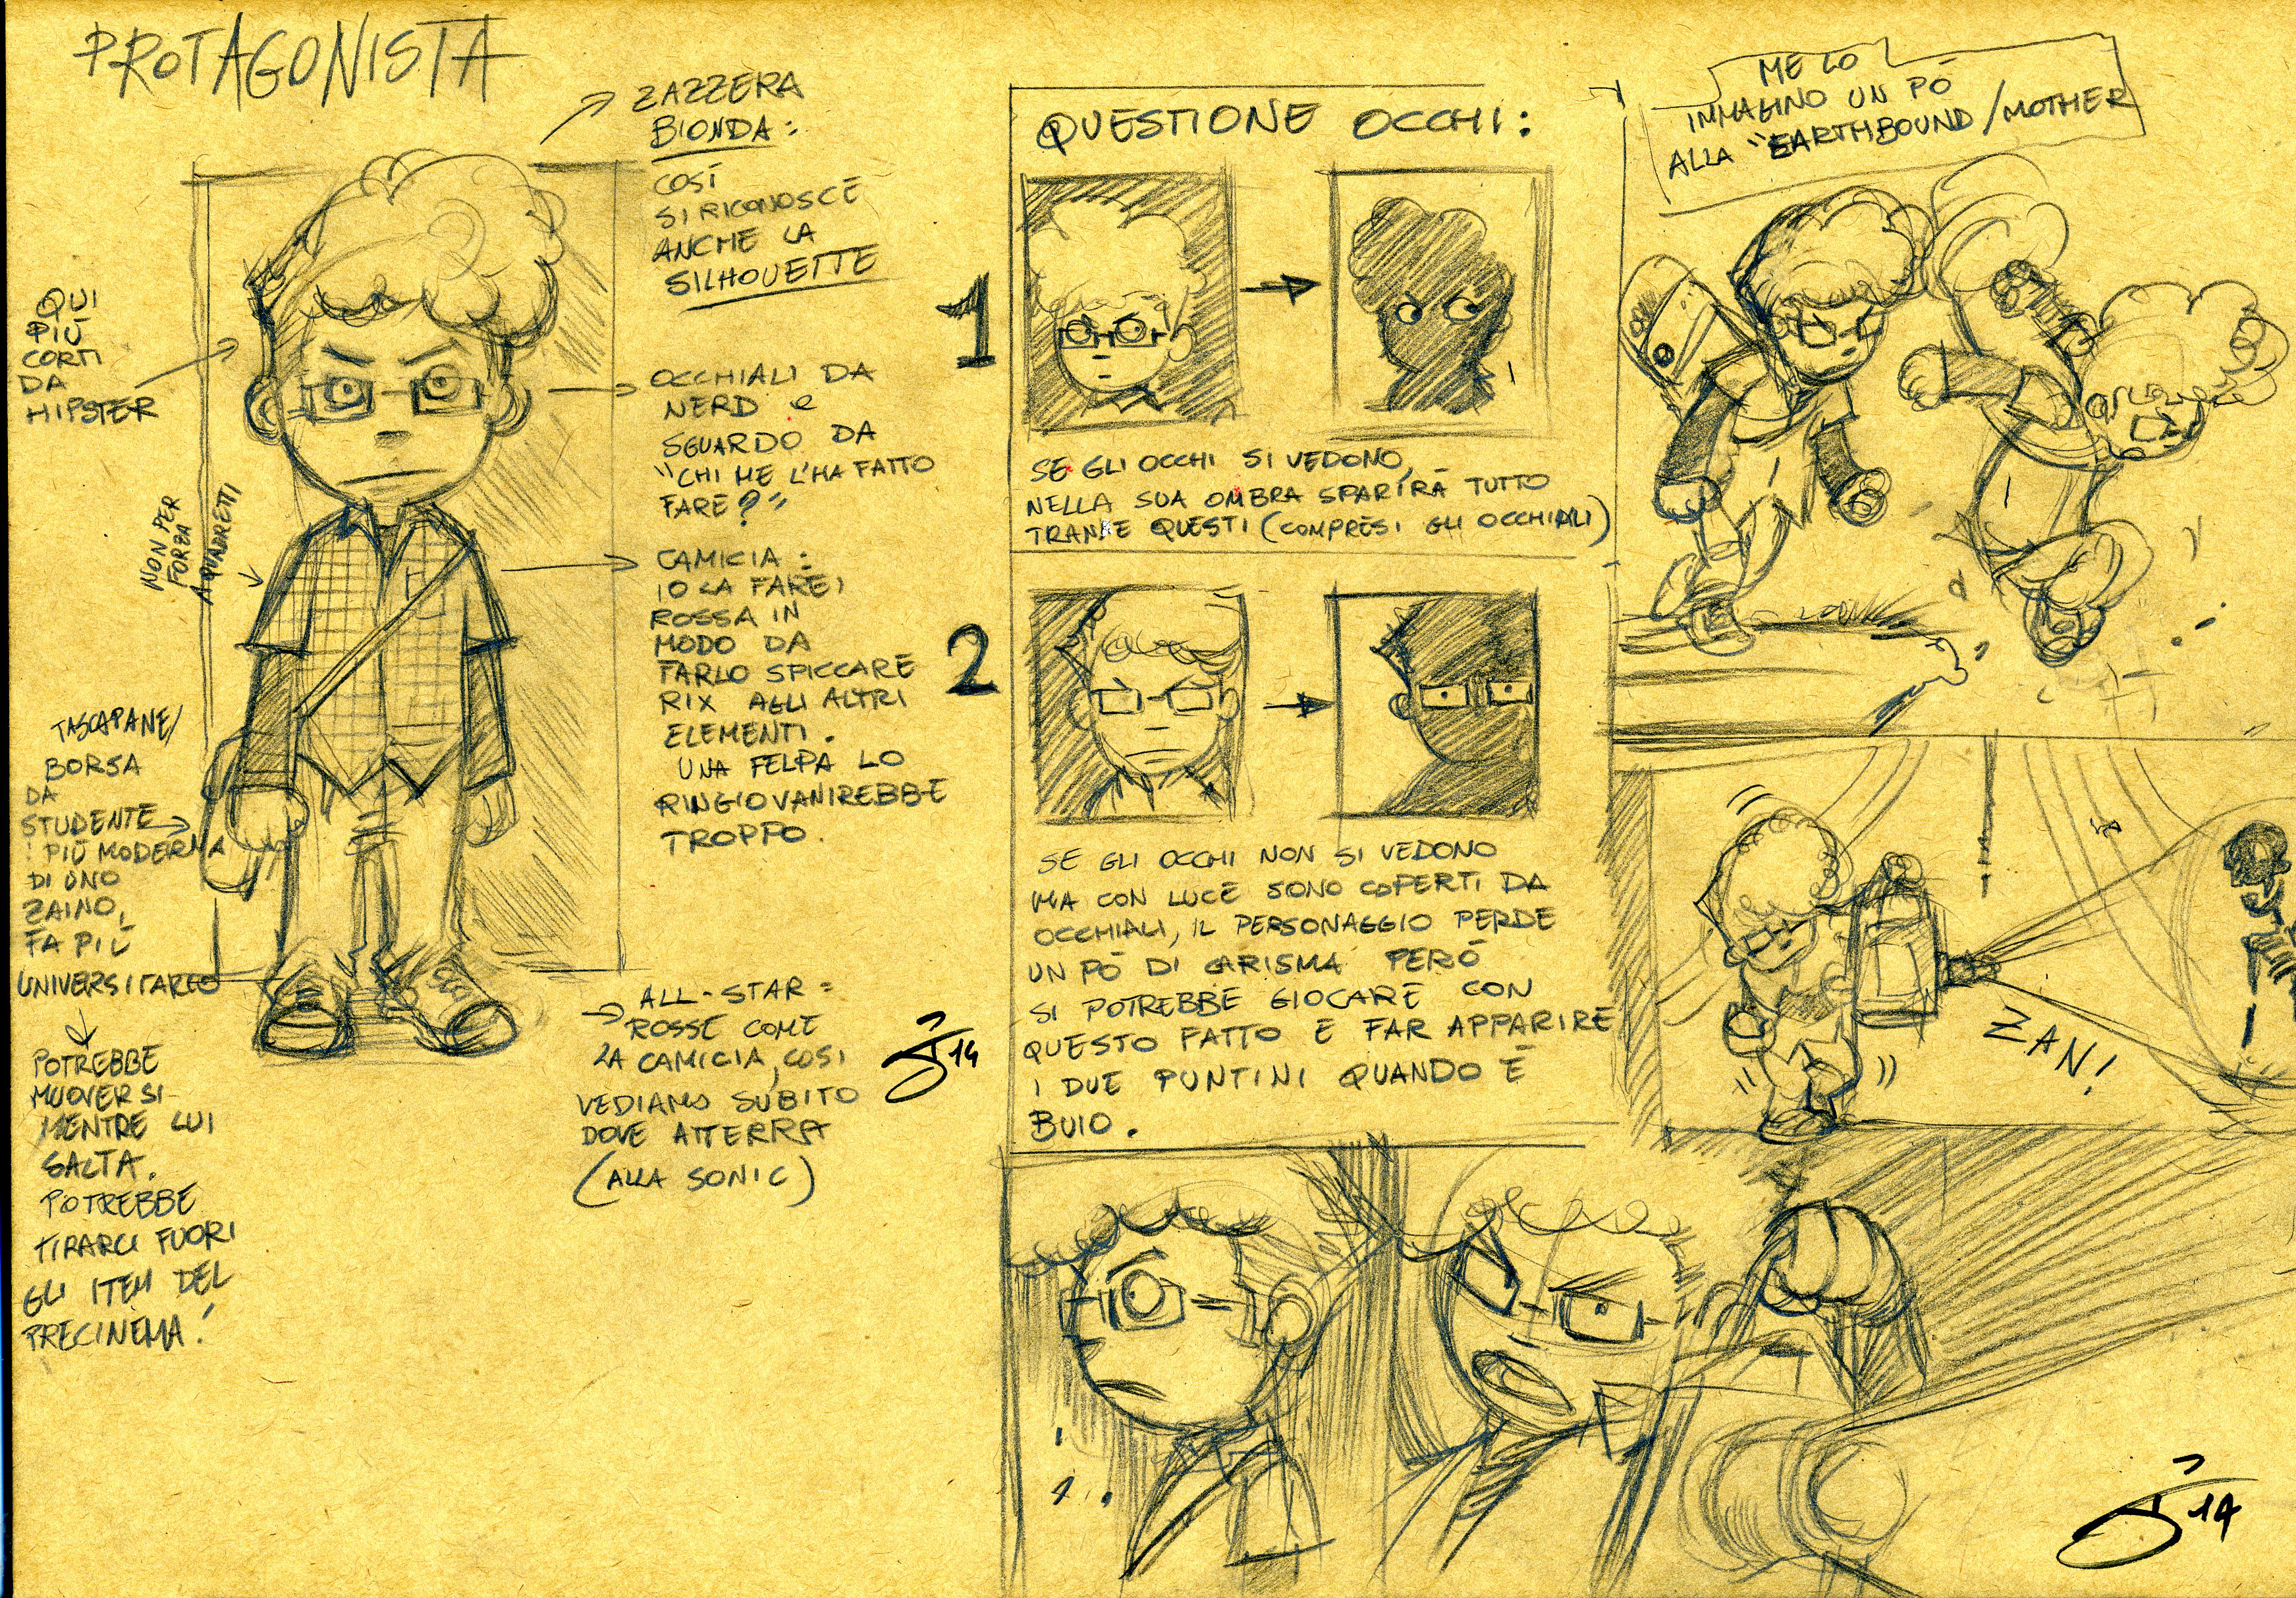
\includegraphics[width= \columnwidth]{images/gameDesign/31_personaggio_02.jpg}
	\caption{Schizzi del personaggio realizzati dal reparto grafico.}
	\label{fig:ambientazione_personaggio_01}
\end{figure} 

Come si può notare, le prime idee sviluppate prevedevano il controllo di un ragazzino, con una caratterizzazione che poteva farlo apparire interessato all’ambito culturale e quindi museale, da notare in particolar modo gli occhiali e la borsa a tracolla da studente. Parallelamente aveva però anche un aspetto molto giovanile e ribelle, sicuramente più attraente per un pubblico giovane. A tal riguardo, sono da sottolineare le scarpe, la camicia fuori dai pantaloni e la maglietta che esce dalla camicia.
Era dipinto con una silouette molto riconoscibile e quindi in possesso di una importante caratterizzazione.

Un personaggio del genere però, non sarebbe risultato molto attinente con le finalità di gioco. Il prodotto prevedeva che il personaggio fosse una trasposizione distorta del giocatore all’interno dell’ambientazione, così da permettere una maggiore immedesimazione. Caratterizzare quindi eccessivamente il personaggio avrebbe rischiato di sortire l’effetto contrario, e quindi allontanare e far percepire più distante il giocatore dal mondo di gioco.

Il passo successivo è stato quindi quello di studiare un nuovo personaggio, ma con caratteristiche più neutre, più impersonali e quindi più adatte allo scopo.
È stata scelta una colorazione scura uniforme, senza eccessivi dettagli, con i due occhi che spiccano decisamente rispetto al corpo. Inizialmente era stato anche ipotizzato di dotare il personaggio di un solo occhio, poi si è accantonata questa ipotesi, per distinguerlo maggiormente dai nemici. Il personaggio può comunque essere dotato di un vestito che possa renderlo più attraente e meno spoglio.

\begin{figure}%[h]
	\centering
	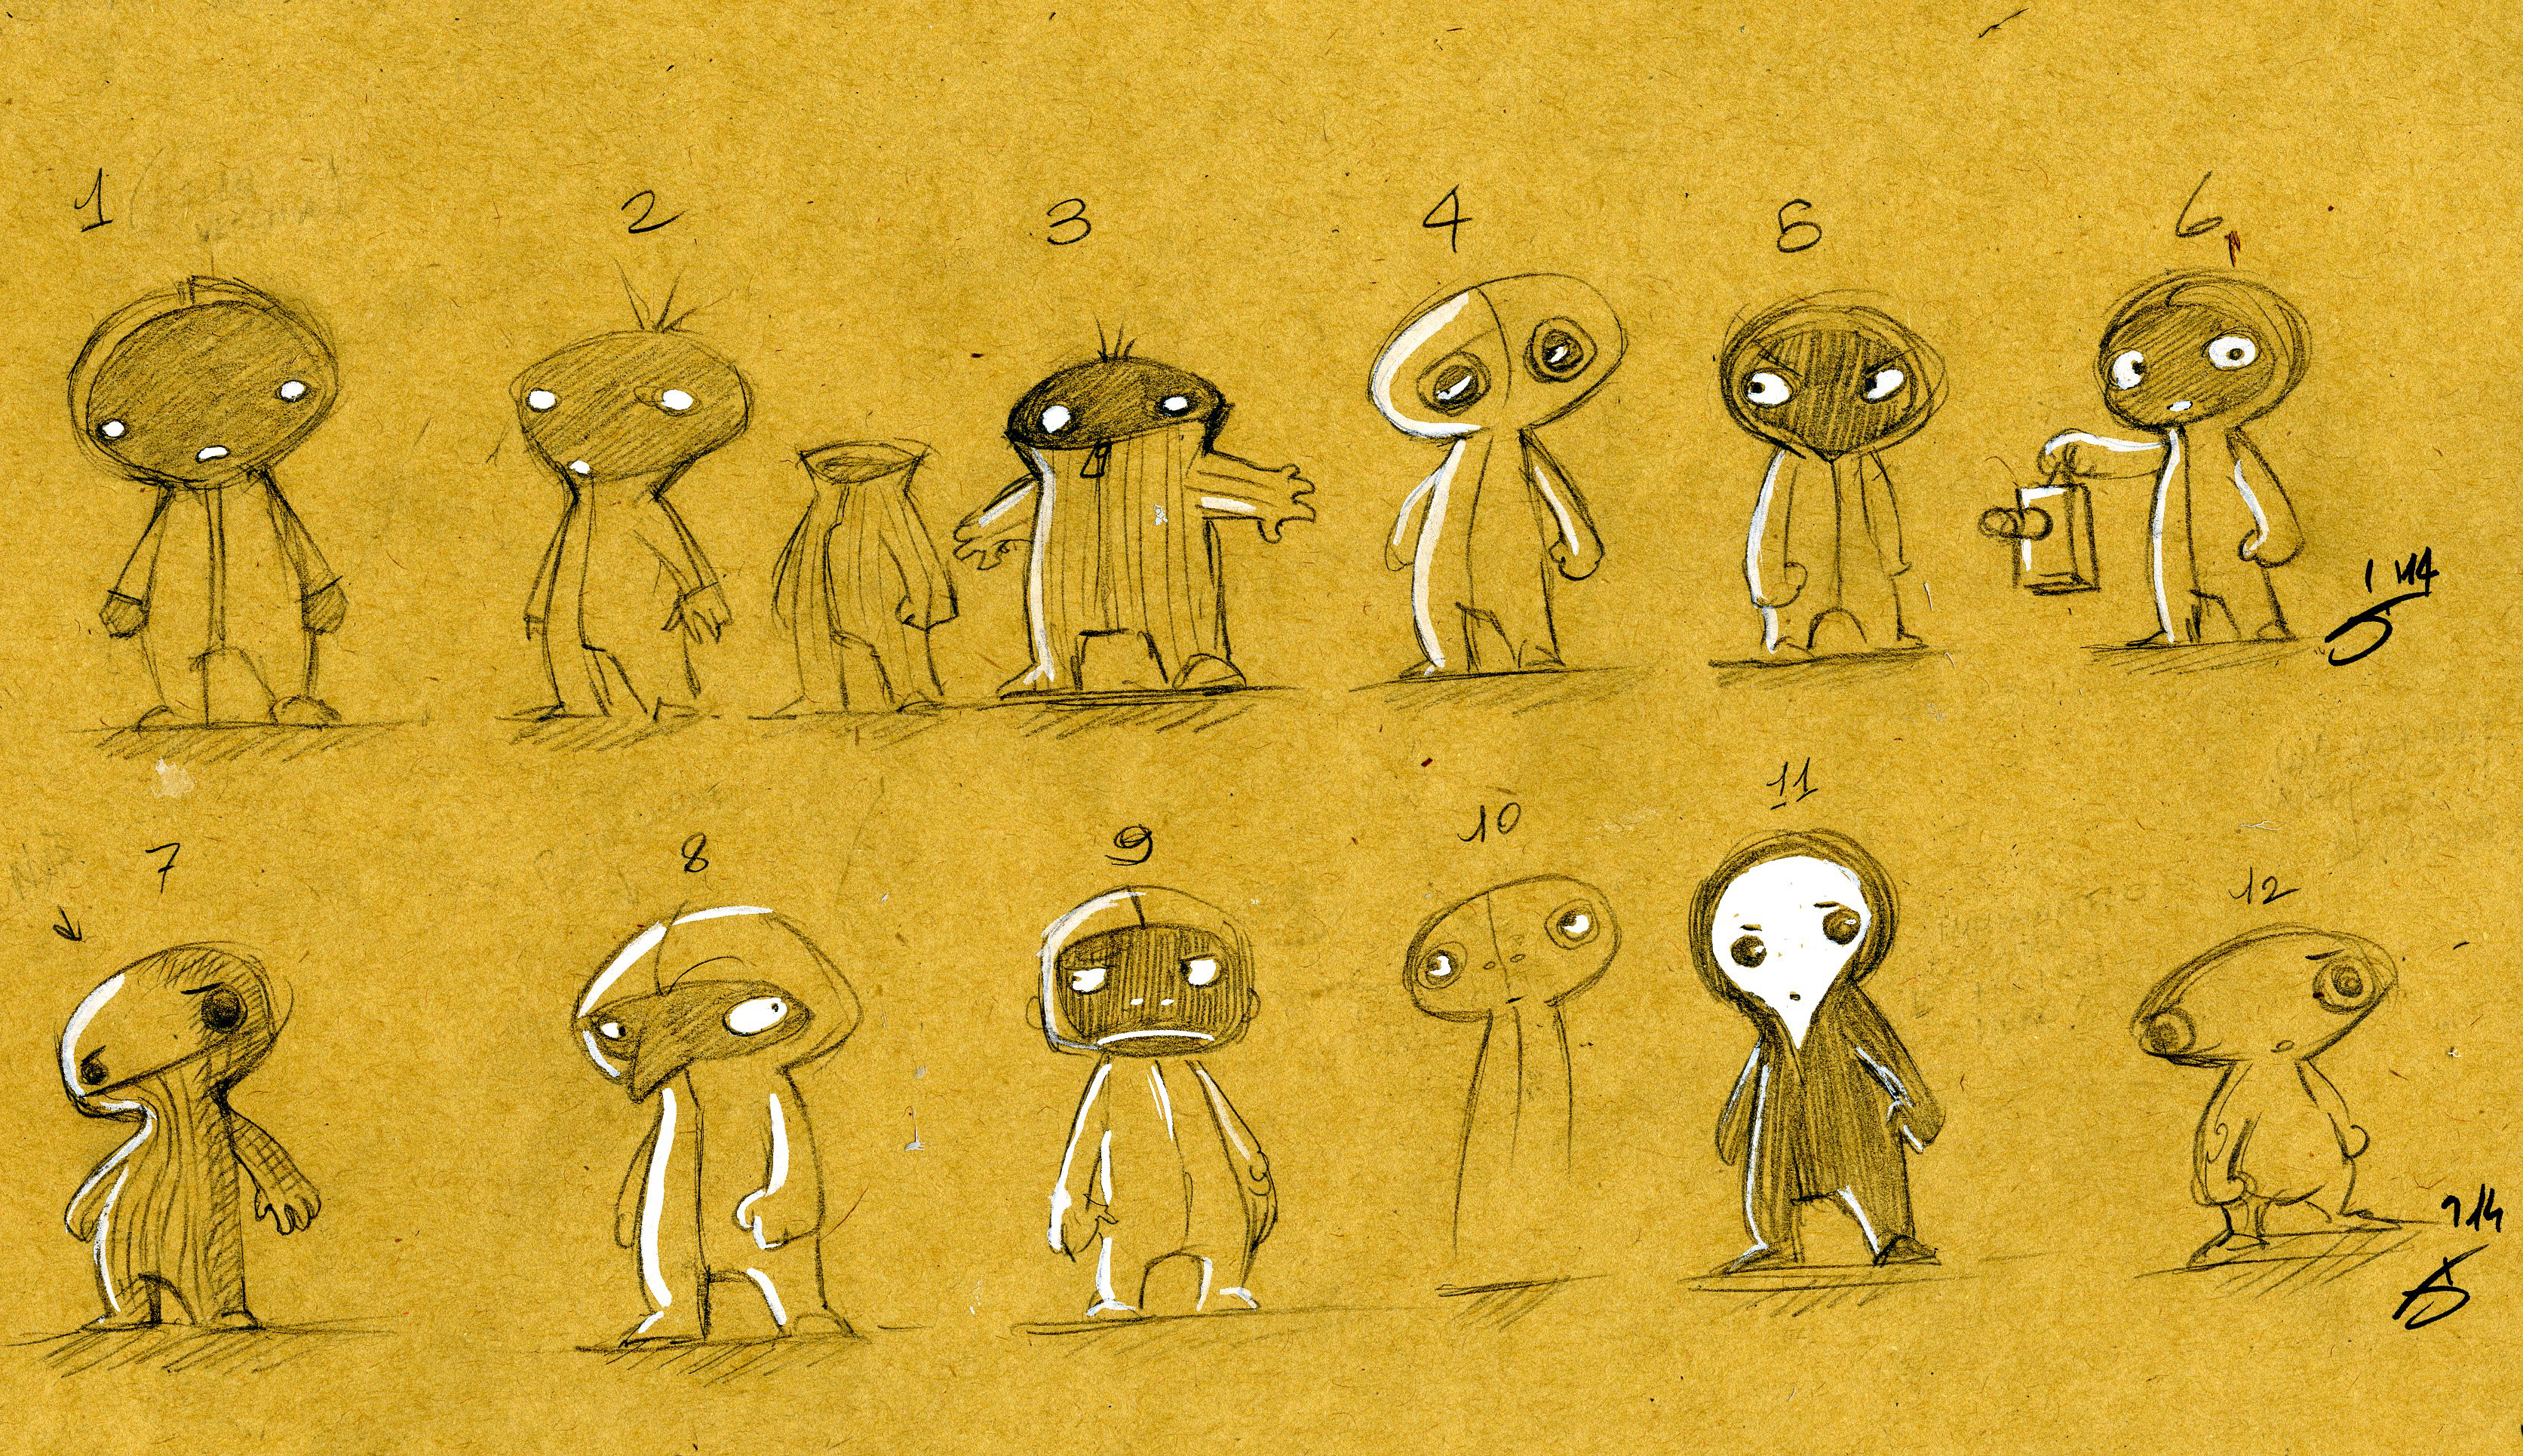
\includegraphics[width= \columnwidth]{images/gameDesign/32_personaggio_03.jpg}
	\caption{Schizzi più impersonali del personaggio realizzati dal reparto grafico.}
	\label{fig:ambientazione_personaggio_02}
\end{figure}

Come già spiegato nel capitolo relativo al design per le ambientazioni, per quanto riguarda gli \textit{asset} sviluppati per il prototipo, ci siamo limitati a quegli elementi essenziali per la comprensibilità, l’usabilità e quindi verifica delle meccaniche di gioco.

Per quanto riguarda il personaggio quindi, abbiamo utilizzato i disegni forniti gratuitamente da David Hellman \cite{DavidHellmanSite} ed utilizzati per il videogioco Braid (Capitolo~\ref{sec:stato_arte_braid}), da lui ideato e sviluppato.
Attualmente quindi, anche per quanto riguarda il personaggio principale, l’aspetto ottenuto, non è attinente con ciò che verrà mostrato nel prodotto finale.

\subsection{Nemici}
\label{sec:nemici}

Per quanto riguarda il design dei nemici si è scelto di caratterizzarli con un solo grande occhio ed un corpo buffo. Poiché le arti di cui trattiamo sono visive, i mostri hanno un occhio grande che possa riportare al concetto di visione. Nel concept iniziale, inoltre, il gioco assumeva una caratteristica molto più \textit{stealth}, con l’utilizzo costante dell’alternanza tra zone illuminate e zone d’ombra, così che l’occhio grande avesse ben potuto rendere l’idea del nemico cacciatore.

Nelle prime versioni del nemico, questo possedeva delle ciglia minacciose che avrebbero dovuto spingere il giocatore a fare attenzione nell’avvicinarsi ad esso (Figura~\ref{fig:ambientazione_nemico_01}).
Il corpo dovrebbe simulare l’idea di una lacrima scura che viene generata dall’occhio stesso.

\begin{figure}%[h]
	\centering
	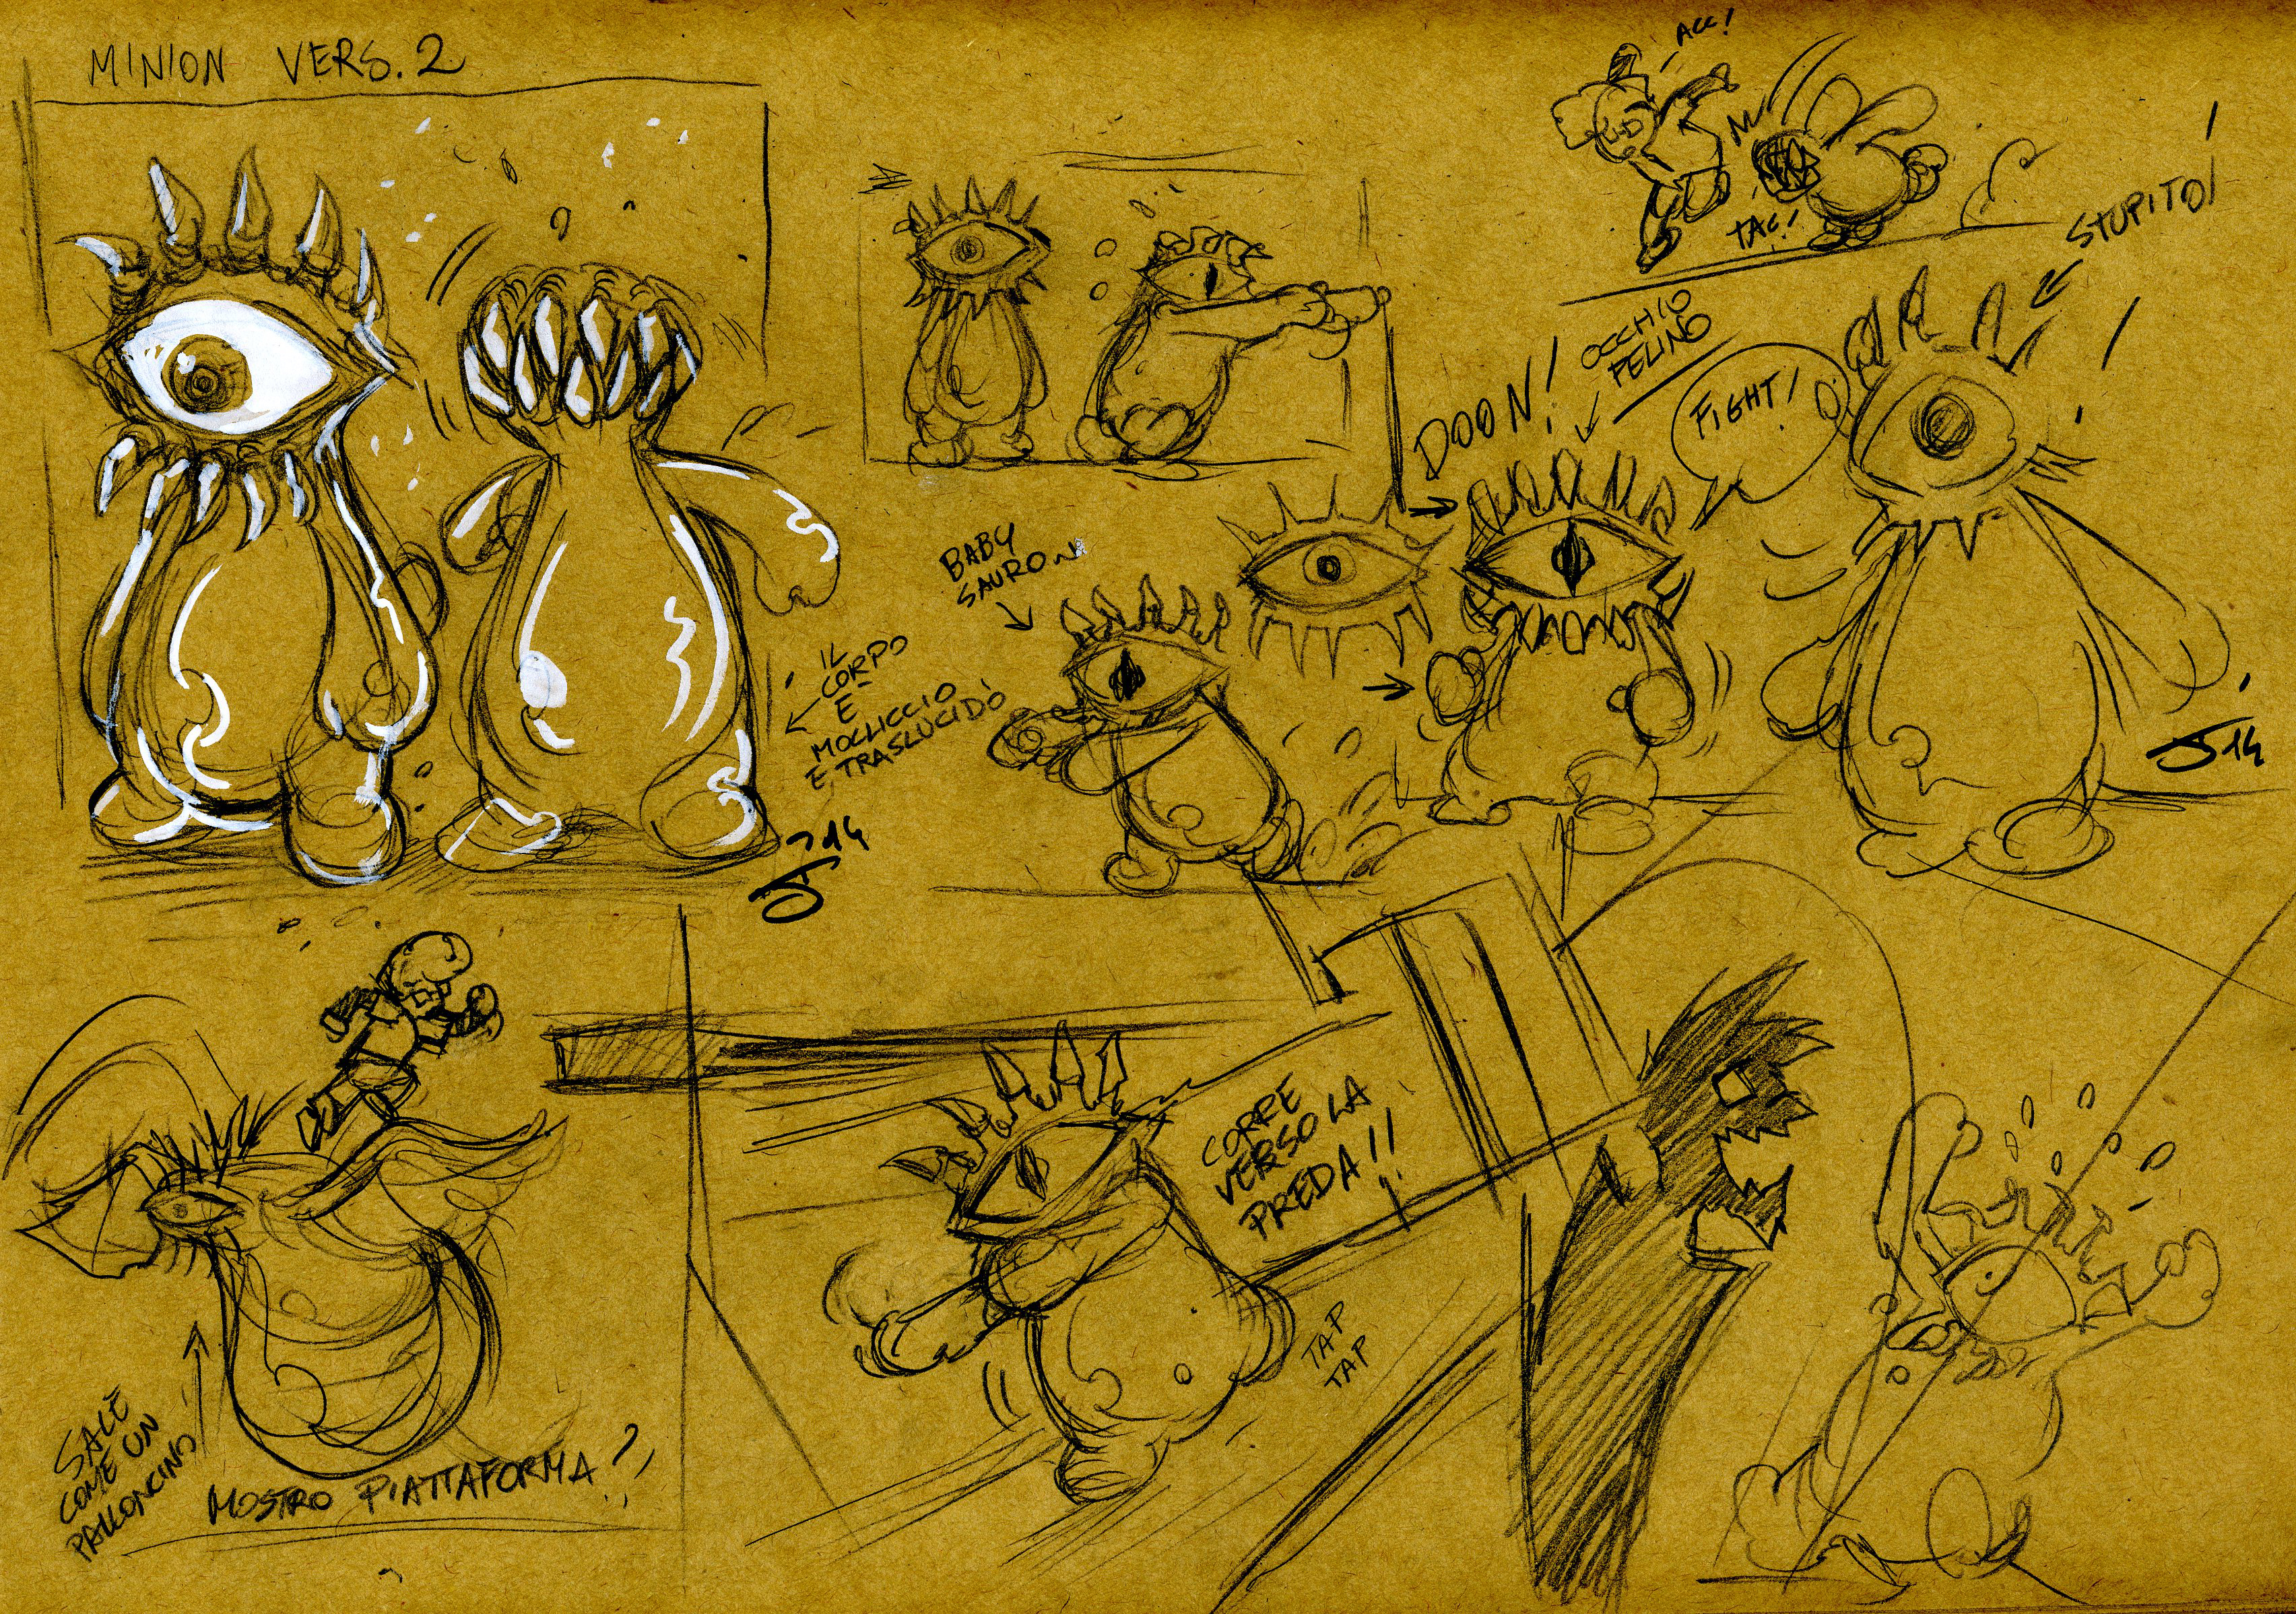
\includegraphics[width= \columnwidth]{images/gameDesign/33_nemici.jpg}
	\caption{Schizzi del nemico realizzati dal reparto grafico.}
	\label{fig:ambientazione_nemico_01}
\end{figure}

L’idea preliminare di concept prevedeva che, mentre il personaggio fosse la trasposizione del giocatore nell’ambiente di gioco, i nemici fossero una rappresentazione astratta degli altri visitatori e di altri elementi del museo.
A partire quindi dall’idea base sono state sviluppate varie tipologie di nemici, osservabili in Figura~\ref{fig:ambientazione_nemico_02}, in ognuna con caratteristiche e comportamenti differenti a seconda della situazione:

\begin{itemize}
	\item \textbf{Minion}. Si tratta del nemico base. Molto goffo e quasi inoffensivo. È la trasposizione dei bambini che visitano il museo.
	\item \textbf{Predatore}. Ha denti più affilati, è più veloce e più intelligente. Trasposizione degli adulti, accompagnatori dei bambini.
	\item \textbf{Spesso}. È alto e con spalle larghe. Ha denti più grossi. È lento ed immune alle trappole. Trasposizione dei guardiani del museo.
	\item \textbf{Volante sentinell}. Un grande occhio alato. Non ha denti e non può ferire, ma avverte gli altri della presenza del personaggio principale. Trasposizione delle telecamere del museo.
	\item \textbf{Volante rapace}. Simile alla sentinella, ma con aspetto più minaccioso. Può ferire. Trasposizione dei piccioni della Mole Antonelliana di Torino.
\end{itemize}

\begin{figure}%[h]
	\centering
	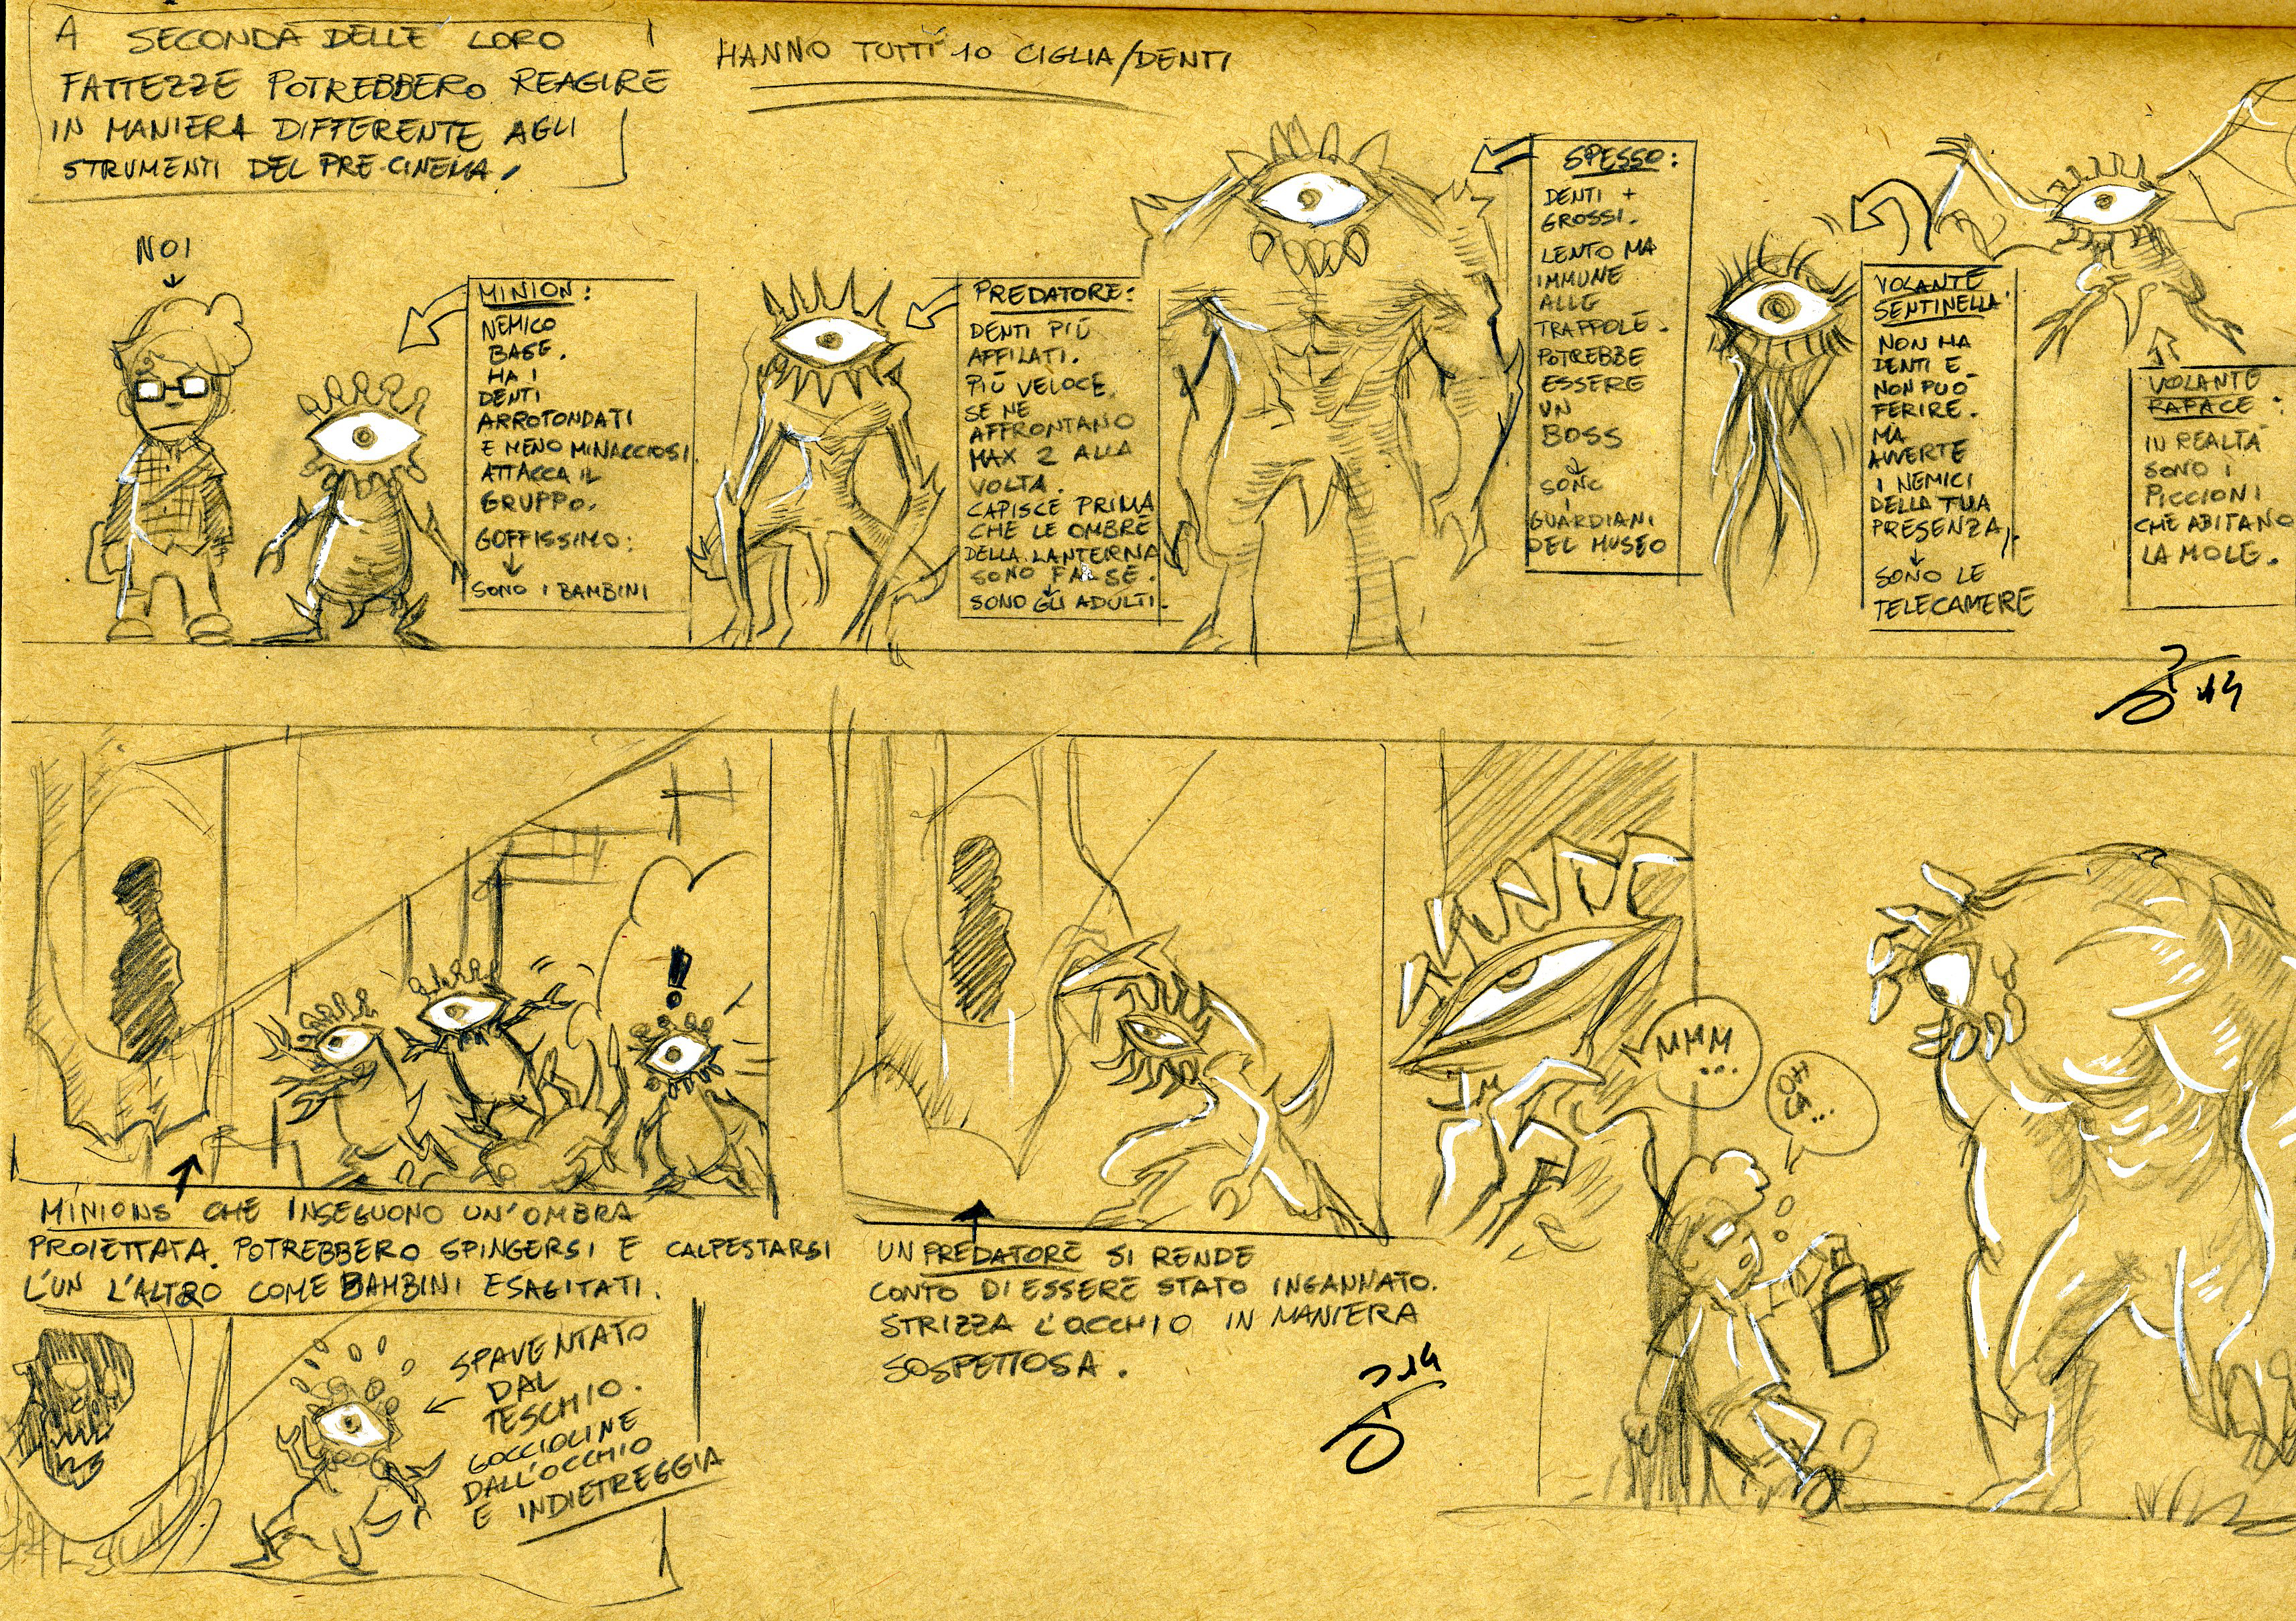
\includegraphics[width= \columnwidth]{images/gameDesign/34_nemici.jpg}
	\caption{Schizzi delle varie tipologie di nemici.}
	\label{fig:ambientazione_nemico_02}
\end{figure}

Una volta delineate le meccaniche principali di gioco e le possibili ambientazioni, è stata quindi analizzata ogni tipologia di nemico, così da studiarne le caratteristiche ed estrapolarne ogni possibile meccanica interessante ai fini del gameplay.

È importante che ogni tipologia di nemico abbia caratteristiche uniche e non sovrapponibili, così da giustificarne l’esistenza e assicurare che il giocatore capisca il modo di approcciare ogni minaccia nel modo appropriato. Risulta fondamentale anche caratterizzarli a livello grafico, così che ogni azione sia giustificata e il comportamento possa essere prevedibile ancora prima che entrino in azione.

In seguito alla fase di design delle principali meccaniche, e dopo aver considerato gli obiettivi primari dello sviluppo del prototipo, abbiamo deciso di utilizzare due tipologie di nemici, visibili in Figura~\ref{fig:ambientazione_nemico_03}:

\begin{itemize}
	\item \textbf{Dumb}. \label{dumb} È un personaggio goffo caratterizzato dall’aver l’occhio chiuso. Avanza fino ad incontrare un ostacolo e quindi torna indietro in un moto continuo. Uccide il personaggio principale al contatto. Può essere ucciso con un salto in testa o nel momento in cui raggiunge elementi danneggianti, come le punte infilzanti. Il salto in testa fornisce al personaggio una spinta verso l’alto.
	\item \textbf{Guard}. \label{guard} Graficamente risulta simile al dumb, se non fosse per un aspetto meno goffo e per l’avere l’occhio aperto. L’occhio suggerisce che controlli una porzione di scenario. Può trovarsi fermo in una posizione o proseguire con un moto simile a quello del dumb. Nel momento in cui vede il player di fronte a lui, entro un determinato raggio, inizia un’animazione di carica. Quando il personaggio esce dal suo campo visivo, risulta spaesato per qualche istante, poi torna alla precedente situazione. Il personaggio viene istantaneamente ucciso al contatto. Può essere stordito da un salto in testa del personaggio. Non viene ucciso se non andando a contatto di un elemento danneggiante, come le punte. Il salto in testa fornisce al personaggio una spinta verso l’alto.
\end{itemize}

\begin{figure}%[h]
	\centering
	\includegraphics[width= 0.8\columnwidth]{images/gameDesign/35_nemici.jpg}
	\caption{Tipologie di nemici utilizzate nel prototipo.}
	\label{fig:ambientazione_nemico_03}
\end{figure}

Il \textit{dumb} è il primo nemico che si incontra, il suo comportamento è facile e prevedibile, viene utilizzato per permettere al giocatore di familiarizzare in maniera intuitiva con i nemici. Viene sfruttato soprattutto per premere pulsanti posti in luoghi non favorevoli al player o per raggiungere luoghi elevati grazie alla possibilità di saltargli in testa. Può essere guidato in diverse sezioni di gioco, ad esempio, cercando di sostituire un eventuale caduta con una proiezione di piattaforma (Paragrafo~\ref{item:piattaforma}) o eliminando un ostacolo, ad esempio aprendo una porta.

Il \textit{guard} è un nemico più difficile da affrontare, in quanto reagisce direttamente alla presenza del nemico. Il moto di carica è più veloce di quello della semplice camminata, oltre che del player stesso, che è perciò costretto a fuggire o saltarlo con repentinità. La differenza principale di gameplay rispetto al \textit{dumb} consiste nel fatto che possa essere “guidato” facilmente in differenti sezioni di gioco, comportamento dovuto alla natura stessa del nemico che tende ad inseguire il personaggio.

\section{Audio e Suoni}
\label{sec:audio}

Per quanto riguarda l’audio presente del gioco, non siamo stati accompagnati da un reparto di esperti. Abbiamo quindi effettuato un design approfondito anche da questo punto di vista. 

Ogni elemento sonoro inserito è stato trovato online, dopo attente ricerche relative alle tematiche ed alle tipologie di suoni necessari. Chiaramente ogni elemento adoperato, è caratterizzato da una licenza gratuita, quindi liberamente utilizzabile per gli scopi del nostro progetto.

Per quanto riguarda la musica presente nei livelli, abbiamo ritenuto opportuno inserire, nell’\textit{hub centrale} (Capitolo~\ref{par:hub_centrale}), un tema che avesse generato sensazioni di sospensione e mistero. Il campione audio inserito è tale per cui la prima sezione risulti differente dalla seconda, caratterizzata invece da toni che generano sorpresa di fronte ai nuovi elementi che vengono mostrati a schermo e scoperti dal giocatore per la prima volta.
Nelle successive visite all’\textit{hub}, che avvengono nella transizione tra i livelli, la musica mantiene comunque una caratterizzazione misteriosa pur adattandosi alle nuove tematiche ascoltate nei livelli.

Questi sono caratterizzati da musiche decisamente più allegre. Il primo livello (Capitolo~\ref{par:livello1}) in particolare possiede un tema musicale molto frenetico ed agitato, che spinge il giocatore ad affrontare le prime sezioni \textit{platform} con spensieratezza, senza porre l’attenzione su elementi troppo impegnativi dal punto di vista della logica di gioco.
Con l’evolversi dei livelli, le musiche diventano decisamente più adatte alle meccaniche \textit{puzzle}, restano comunque luminose ed allegre, ma decisamente meno frenetiche di quella ascoltata nel primo livello. Tali temi tendono a rilassare il giocatore, pur mantenendo alta la sua attenzione durante le sezioni che richiedono maggiori abilità di ragionamento.

\section{Level Design}
\label{sec:level_design}

Per \textit{Level Design} si intende la creazione dell’ambiente di gioco a partire dalle meccaniche che si è deciso di includere. È un elemento di fondamentale importanza nella creazione di un prodotto videoludico. Senza un buon \textit{Level Design} l’esperienza può risultare noiosa e poco stimolante o eccessivamente frustrante, anche in presenza di ottime meccaniche di gioco.

\subsection{Principi di Level Design}
\label{sec:principi_level_design}

Nell’affrontare il design dei livelli sviluppati, abbiamo cercato di seguire dei passi che ci avessero permesso di ottenere i risultati prefissati, in modo ordinato.
La prima fase è quella di cercare di elencare ogni elemento che deve essere presente nel livello. Con “elemento” non si intendono solo gli oggetti che popolano lo scenario, ma anche quello che il giocatore deve riuscire ad imparare, a padroneggiare e le sfide di fronte a cui si deve porre. A titolo di esempio vengono riportati alcuni obiettivi che ci siamo posti per il primo livello:

\begin{itemize}
	\item Il giocatore deve imparare ad usare i tasti direzionali per muoversi.
	\item Deve imparare ad usare il salto.
	\item Deve padroneggiare la meccanica del salto.
	\item Deve capire che, attraverso l’utilizzo del puntatore, può osservare altre sezioni di gioco.
	\item Deve capire e dare per scontate le differenze tra le varie tipologie di terreno.
\end{itemize}

Una volta chiariti quali devono essere gli obiettivi, si inizia a disegnare su carta alcune sezioni che permettono di raggiungere lo scopo prefissato. Ogni sezione viene quindi analizzata attentamente per capire eventuali criticità, se sia necessario farla precedere da una sezione più facile con lo stesso scopo, se possa risultare troppo difficile per il livello scelto.

Dopo aver creato un buon numero di porzioni di livello si prova ad assemblarlo ed analizzarlo nel suo complesso per capire se ci sia necessità di inserire nuove sezioni o eliminarne di esistenti.
È in questo punto che risulta fondamentale il discorso già intrapreso in altri capitoli riguardo il cercare di mantenere l’utente nella situazione di \textit{flow} (Figura~\ref{fig:level_design_flow}). È infatti in questi momenti, in cui il giocatore non è annoiato o frustrato, che si possono ottenere, come risultati:

\begin{itemize}
	\item Estrema attenzione sull’obiettivo.
	\item Senso di controllo dell’azione.
	\item Sinergia tra azione e consapevolezza.
	\item Immedesimazione.
	\item Distorsione dell’esperienza del tempo.
	\item La ricerca dell’obiettivo che spinge a continuare.
\end{itemize}

\begin{figure}%[h]
	\centering
	\includegraphics[width= 0.8\columnwidth]{images/gameDesign/36_flow.jpg}
	\caption{Rappresentazione grafica della situazione di Flow.}
	\label{fig:level_design_flow}
\end{figure}

Per far sì che il giocatore mantenga queste condizioni, è necessario che il livello accompagni l’utente lungo una curva di apprendimento che gli permetta di comprendere con facilità le meccaniche di gioco, di aumentare progressivamente il livello di difficoltà e permettere quindi un padroneggiamento delle meccaniche che generi soddisfazione e gratificazione.
È quindi necessario un attento studio degli elementi di gioco e degli equilibri che si devono venire a creare lungo la progressione del livello.
Una volta che si ha l’idea della struttura generale del livello, questo viene testato a fondo e modificato di conseguenza, in modo da perfezionare ogni dettaglio dell’esperienza di gioco, assicurandosi che gli obiettivi, che si erano descritti nella fase iniziale del \textit{Level Design}, siano stati raggiunti.
I passi che abbiamo seguito, e precedentemente descritto, sono in parte ispirati dall’articolo di Diorgo Jonkers, “How to design levels for a platformer” \cite{DiorgoJonkersArticle}.

Anche il libro The Art Of Game Design \cite{artOfGameDesign}, di Jesse Schell, fornisce alcuni interessanti spunti a riguardo, che ci hanno aiutato nella creazione delle varie sezioni di gioco.

La prima idea che emerge dall’analisi del capitolo “Game Mechanics Support Puzzles” è che i puzzles sono ovunque in un videogioco, spesso sono visibili e mostrati come tali, altre volte sono insiti nel gameplay, così da sembrare nascosti. Jesse Schell definisce puzzle ogni elemento di gioco che faccia fermare e pensare. Anche i giochi puramente action possiedono un gran numero di componenti puzzle, basti pensare ad una possibile battaglia con un boss di gioco. Il riuscire a capire il suo punto debole e come sfruttarlo a proprio vantaggio è un elemento puzzle. In un gioco di corse in cui si cerca di capire come superare l’avversario e si decide di sfruttarne la scia per ottenere una maggiore velocità, si sta risolvendo un puzzle. Ogni sezione di gioco che richieda l’utilizzo di una meccanica, in maniera non scontata, ha una componente puzzle.

Con l’evolversi dei videogiochi c’è stato un graduale passaggio dal puzzle esplicito a quello implicito, ma è esclusivamente dovuto al cambiamento di gusti dei giocatori ed alla maturazione delle abilità dei game designers.
L’autore ha definito dei principi, che abbiamo ritenuto fondamentali nello sviluppare ed architettare in maniera armoniosa tutti i livelli di gioco, di cui riportiamo di seguito una personale traduzione:

\begin{itemize}
	\item \textbf{Rendere l’obiettivo facile da capire.} Per fare in modo che i giocatori siano interessati, devono sapere cosa ci si aspetti che facciano.
	\item \textbf{Deve essere facile iniziare.} Una volta che il giocatore capisce l’obiettivo del puzzle, inizia a risolverlo. E con alcuni puzzle, è abbastanza chiaro come iniziare, sebbene non sia ovvio come risolverlo.
	\item \textbf{Dare un senso di progressione.} Ai giocatori piace la sensazione di fare progressi nel risolvere una situazione, dà loro speranza di stare arrivando alla risposta.
	\item \textbf{Dare un senso di risolvibilità.} Se il giocatore inizia a dubitare del fatto che un puzzle sia risolvibile, può diventare preoccupato del fatto di star perdendo tempo. Un modo per assicurarsi che ciò non avvenga è appunto mostrare dei progressi.
	\item \textbf{Aumentare gradualmente la difficoltà.} Abbiamo analizzato più volte questo punto. È un discorso che va molto al di là del singolo puzzle. In questo caso si intende la crescente difficoltà nel proporre al giocatore puzzle simili ma con soluzioni sempre più difficili, che lo invitino a superare i limiti raggiunti precedentemente.
	\item \textbf{Parallelizzare fa riposare il giocatore.} I puzzle, come già detto, fanno pensare a ragionare. C’è perciò il rischio concreto che un giocatore, incapace di fare progressi, abbandoni il gioco. Un buon modo per evitare questo comportamento è fornire contemporaneamente differenti puzzle, così che l’utente possa dedicarsi ad uno di questi e, nel caso dovesse fermarsi troppo a lungo, potersi dedicare ad un altro.
	\item \textbf{Un struttura a piramide estende l’interesse.} Significa che un insieme di piccoli puzzle, ognuno dei quali fornisce un piccolo indizio riguardo un puzzle più grande, aumentano l’interesse del giocatore. In questo modo è facile fornire dei piccoli obiettivi, raggiungibili più facilmente, che concorrono al raggiungimento di un obiettivo maggiore.
	\item \textbf{Gli aiuti estendono l’interesse.} Quando un giocatore sta per abbandonare un puzzle perché troppo difficile, fornirgli un aiuto può rinnovare la sua speranza e curiosità.
	\item \textbf{Dare la risposta.} Spesso basta far ragionare il giocatore e dare una risposta differente al puzzle. L’utente trova soddisfacente il momento in cui la risposta gli viene rivelata, anche se lui era arrivato ad una diversa conclusione. È lo stesso ragionamento che viene fatto per i libri, il lettore può immaginare un finale, ma è l’autore che fornisce la risposta e può essere completamente diversa da quella che si aspettava il lettore. Questo mezzo, se usato attentamente, può dare molta soddisfazione all’utente, portandolo ad incuriosirsi attraverso la sorpresa.
	\item \textbf{I “cambiamenti percettivi” sono un’arma a doppio taglio.} Per cambiamenti percettivi si intendono quei momenti in cui, osservando un determinato puzzle, si riesce a scoprire improvvisamente la soluzione, magari semplicemente cambiando prospettiva o attraverso un’idea inaspettata. Questo tipo di puzzle rischiano di portare a frustrazione il giocatore, in quanto si ottiene una grande soddisfazione nel caso si riesca a risolverlo, ma c’è un grande rischio che questo non avvenga, se, appunto, non si riesce ad avere l’idea giusta.
\end{itemize}

Come si vedrà nell’analisi dei livelli (Capitolo~\ref{sec:analisi_livelli}) i concetti appena espressi hanno fornito una perfetta base per la creazione e lo sviluppo dei livelli di gioco.

\subsection{Scelte relative alla struttura dei livelli}
\label{sec:struttura_livelli}

Nelle prime fasi di Design si è deciso di strutturare l’esperienza di gioco in due fasi ben distinte. All’avvio della partita il giocatore si sarebbe trovato all’interno del museo. L’ambientazione sarebbe stata interamente in 3D, con la possibilità di controllare in prima persona il proprio personaggio. La visita al museo sarebbe dovuta proseguire in maniera lineare lungo un percorso standard. Sarebbero state presenti quindi teche con oggettistica e relative descrizioni.
All’interno dell’ambiente però, alcuni elementi avrebbero permesso al giocatore di infrangere delle regole e perciò uscire dalla visita standard, come una porta con scritto “Staff Only” (Figura~\ref{fig:level_design_staffonly}) o una teca con cui poter interagire per aprirla.

\begin{figure}%[h]
	\centering
	\includegraphics[width= 0.8\columnwidth]{images/gameDesign/37_museo3d.jpg}
	\caption{Rappresentazione tridimensionale del museo ipotizzata nelle prime sessioni di Design.}
	\label{fig:level_design_staffonly}
\end{figure}

Nel momento in cui il player avesse commesso quindi un’azione non prevista dalle regole dal museo, sarebbe entrato in un mondo parallelo, interamente bidimensionale, in cui sarebbero stati presenti la sua trasposizione e quella di tutti gli altri visitatori del museo.
L’ambientazione avrebbe dovuto rispecchiare gli spettacoli dell’epoca del pre-cinema, ispirandosi quindi, sia per meccaniche che per rappresentazione, all’oggettistica di riferimento.
Il capitolo \ref{sec:ambiente_personaggi} affronta in maniera approfondita l’analisi del design di ambientazioni e dei personaggi.

Dopo un’attenta analisi, si è preferito eliminare la prima sezione di gioco in prima persona, perché il passaggio alla seconda non sarebbe stato così immediato, oltre che rischioso da un punto di vista del messaggio comportamentale che avrebbe potuto trasmettere.

Si è quindi deciso di fare in modo che l’esperienza del giocatore non fosse direttamente collegata all’idea di museo, ma che ne richiamasse alcuni aspetti in maniera indiretta.
L’avventura avrebbe quindi assunto una caratterizzazione differente, con connotazioni pesantemente esperienziali. Si è pensato di abbandonare l’idea di sviluppare una ricca componente di \textit{storyline}, ma far sì che l’esperienza vissuta dal giocatore fosse data dall’immersività nel mondo di gioco e dalle sensazioni che questo gli avesse potuto trasmettere.
Per questo tipo di approccio ci siamo in parte ispirati a videogiochi come LIMBO, in cui si controlla un ragazzino, di cui si intuisce solo la sagoma. Ci si trova in un mondo, che ha l’aspetto di una foresta, ricco di pericoli, che metteranno a rischio l’incolumità del personaggio (Figura~\ref{fig:level_design_limbo}). Non è chiaro il perché il ragazzo si trovi in una tale situazione, ma è evidente che deve cercare di uscirne. L’esperienza di gioco è data appunto dalle sensazioni provate dal giocatore, garantite da un’ambientazione ricca di fascino e da meccaniche efficaci.

\begin{figure}%[h]
	\centering
	\includegraphics[width= 0.8\columnwidth]{images/gameDesign/38_limbo.jpg}
	\caption{Screenshot del videogioco Limbo.}
	\label{fig:level_design_limbo}
\end{figure}

\paragraph{Hub centrale.}
\label{par:hub_centrale}
L’utilizzo di collezionabili e di stelle da poter raccogliere nei vari livelli, ha fatto emergere la necessità di fornire al giocatore un mezzo per poter controllare quali fossero stati completati o meno e quindi un modo per potervi accedere in maniera veloce intuitiva.
Si è quindi deciso di sviluppare un \textit{hub centrale} da cui poter raggiungere i vari livelli sviluppati.

Il player quindi, all’uscita di ogni livello si ritrova nell’hub. Da qui può accedere al livello successivo o può controllare il grado di completamento dei livelli già affrontati, così da decidere se rigiocarli o meno.
Come possibile vedere in Figura~\ref{fig:rigiocabilita_UI_hub}, al passaggio di fronte alla porta di accesso di ogni livello vengono quindi mostrate delle barre laterali che indicano il numero di stelle e di collezionabili raccolti.

Inoltre, attraverso l’utilizzo dell’hub, è stato possibile pensare ad un modo efficace di giustificare il raccoglimento di stelle durante l’attraversamento dei livelli.
Attualmente, in tale scena di raccordo, sono presenti degli strumenti, le \textit{lanterne mammut}, che possono essere accese solo se si riesce a soddisfare dei requisiti minimi per quanto riguarda il raccoglimento delle stelle.
Le 4 lanterne mammut poste in 4 angoli dello schermo proiettano in una stessa porzione di scena, che conterrà quindi la sovrapposizione delle immagini di tutte le lanterne. Un utilizzo tipico delle lanterne magiche era appunto quello di sovrapporre vetrini, ognuno con delle sezioni trasparenti, così da ottenere immagini composite più complesse.

L’utilizzo di tale immagine composta è ancora in fase di design. Si sta pensando di sfruttarle per la componente di \textit{storyline}. È necessario quindi studiare 4 vetrini che, sovrapposti progressivamente, possano fornire un’evoluzione visiva di un tema o una situazione che si intende trattare.
L’ultimo vetrino deve essere studiato in modo che fornisca uno stravolgimento del tema, così da stupire il giocatore e giustificare il raccoglimento di tutte le stelle.

\begin{figure}%[h]
	\centering
	\includegraphics[width= \columnwidth]{images/gameDesign/40_premi.jpg}
	\caption{Progressione delle ricompense ottenibili nell'hub centrale.}
	\label{fig:level_design_ricompense}
\end{figure}

Chiaramente tale sviluppo richiede un pesante sforzo di design oltre che un apporto artistico attivo e di buon spessore.
Come è possibile vedere in Figura~\ref{fig:level_design_ricompense}, attualmente le immagini componibili sono strutturate secondo questa progressione, che non rispecchia l’idea proposta precedentemente, e che quindi saranno differenti nel prodotto finale:
\begin{itemize}
	\item Ambientazione misteriosa, un bosco, con la luna che traspare tra gli alberi, una strana foschia e tutto caratterizzato da colorazioni scure.
	\item All’interno dell’ambientazione compare un mago che sta leggendo un giornale, apparentemente nella sua stanza.
	\item La stanza del mago è in realtà una strana struttura che genera luce da un foro nella parte anteriore ed il fumo del camino visto nell’immagine precedente esce da uno strano comignolo.
	\item Compare una mano che fa capire che lo strumento non è nient’altro che la lanterna magica. Cambiano perciò le proporzioni di quello che veniva spiegato in precedenza. Il mago è il mezzo che permette alla lanterna magica di funzionare.
\end{itemize}

La prima implementazione del gioco prevedeva lo sviluppo di 3 livelli, il primo dei quali, con la presenza di un tutorial di movimento e quindi la presentazione delle meccaniche \textit{platform} oltre che di un loro approfondimento. Al termine del livello si sarebbe arrivati quindi per la prima volta all’hub, e da qui la possibilità di proseguire per il secondo livello, oppure controllare i collezionabili raccolti nel primo o provare ad interagire con le lanterne mammut presenti nella scena.
Questo approccio avrebbe quindi catapultato il giocatore immediatamente nel primo livello. Successivamente abbiamo valutato la possibilità di introdurre una piccola porzione di gioco che avrebbe permesso di presentare il prodotto, prima ancora di conoscere e familiarizzare con le vere meccaniche.
L’hub è stato quindi esteso, prevedendo l’inclusione di una sezione iniziale, in cui è presente un piccolo tutorial di movimento. Il giocatore arriva quindi, attraverso una tenda da cinema, nell’hub vero e proprio dove, al centro della stanza, viene proiettato il titolo \textit{“The Magic Lantern”}. Da qui è perciò possibile accedere al primo livello e dare inizio alla partita.

\subsection{Analisi dei livelli}
\label{sec:analisi_livelli}

Il prototipo è strutturato in 3 livelli. Nel primo vengono presentate le meccaniche \textit{platform}, il secondo è quello in cui si raccoglie la lanterna magica e quindi c’è la presenza del vero \textit{game-changer}, mentre il terzo mostra le vere potenzialità della lanterna magica attraverso un utilizzo più curioso.

Verranno di seguito analizzati i 3 livelli in dettaglio. È importante ricordare che, poiché sono state effettuate due fasi di testing del prodotto (Capitolo~\ref{chap:testing}), questo ha assunto due forme leggermente diverse. Per il secondo testing infatti, sono state corrette alcune sezioni ed altre sono state accantonate, seppur ritenute di buon valore, per mettere in evidenza solamente gli elementi che abbiamo ritenuto opportuno sottolineare durante il test. Alcune sezioni analizzate in seguito potrebbero essere presenti nella prima versione del prototipo ed essere assenti nella seconda, o viceversa.

\paragraph{Livello 1}
\label{par:livello1}

Come già detto, il primo livello viene utilizzato con la funzione di tutorial di movimento oltre che di presentazione e padroneggiamento di tutte le meccaniche \textit{platform} che verranno utilizzate anche nei livelli successivi.
Nella prima sezione viene insegnata al giocatore la meccanica del salto, tramite un piccolo ostacolo da superare ed un comando visibile a schermo, come mostrato in Figura~\ref{fig:livello1_salto}.

\begin{figure}%[h]
	\centering
	\includegraphics[width= 0.8\columnwidth]{images/gameDesign/41_salto.jpg}
	\caption{Livello 1. Primo salto.}
	\label{fig:livello1_salto}
\end{figure}

Successivamente viene testato se il giocatore ha appreso correttamente l’utilizzo della meccanica attraverso dei semplici salti, che mostrano come possa essere usata sia per superare ostacoli in altezza, che per attraversare piattaforme separate tra loro in lunghezza.

A questo punto, considerando i problemi riscontrati da alcuni ragazzi durante il primo test, abbiamo ritenuto necessario inserire anche una piccola sezione in cui insegnare come utilizzare le scale. È quindi presente una scala che permette di raggiungere una piattaforma, con il relativo comando mostrato a schermo.

Successivamente, viene mostrata per la prima volta la meccanica del bottone e della porta, oltre che l’utilizzo intuitivo di una cassa, come si può osservare in Figura~\ref{fig:livello1_bottone}. Il bottone si trova in una zona sottostante la porta da attraversare. Il giocatore può scendere, premere il bottone e notare la porta che si apre, una volta sceso dal bottone nota la porta chiudersi. La presenza della cassa induce il giocatore a spingerla sul bottone così da mantenerlo premuto. La cassa può quindi essere utilizzata per raggiungere la porta, posta in un posto troppo in alto. Questo semplice puzzle nasconde un intelligente lavoro di \textit{Level Design}. 

L’utilizzo di un semplice bottone per aprire una porta non avrebbe impresso bene nella mente del giocatore il suo funzionamento, nel modo proposto invece, si è costretti ad un ragionamento che spinge all’utilizzo di uno strumento presente a schermo, la cassa, per raggiungere l’obiettivo prefissato. L’utilizzo della cassa per tornare alla zona più elevata è un rafforzativo della meccanica del salto oltre che un efficiente modo per mostrare il limite massimo raggiungibile in altezza con un salto del personaggio.

\begin{figure}%[h]
	\centering
	\includegraphics[width= 0.65\columnwidth]{images/gameDesign/42_bottone.jpg}
	\caption{Livello 1. Primo bottone, accompagnato dalla cassa.}
	\label{fig:livello1_bottone}
\end{figure}

Successivamente sono state poste 3 piccole sezioni, mostrate in Figura~\ref{fig:livello1_verifiche_salto} che fungono da rafforzativo della meccanica del salto. 

Nella prima vengono poste 2 piattaforme in obliquo, è necessario quindi valutare le possibilità della meccanica sia per quanto riguarda lo spostamento in altezza, che quello laterale. Sotto le piattaforme sono poste delle punte. È il primo momento in cui il personaggio possa morire. Poco prima delle piattaforme è quindi posto un punto di salvataggio per non far perdere troppo tempo al giocatore. Questa sezione è molto importante perché, mentre risulta fondamentale presentare la nuova meccanica in uno stato di sicurezza per il personaggio, questa va perfezionata aggiungendo progressivamente difficoltà, che stavolta consiste nella possibilità di morire.

Nella breve sezione successiva viene proposto un nuovo salto, simile ai due precedenti, solo che, questa volta la piattaforma è proiettata da una lanterna magica che si accende e si spegne ad intermittenza. Lo scopo è quindi duplice, quello di testare le capacità di reazione e tempismo del giocatore, oltre che di presentare un elemento di gioco curioso, che solo nelle sezioni più avanzate di gioco potrà essere controllato e sfruttato a proprio piacimento.

Nella sezione successiva viene portato al limite il concetto di salto, proponendo una struttura simile a quelle già analizzate, quindi familiari al giocatore, ma stavolta le piattaforme sono molto più strette, richiedono quindi un controllo ed un’attenzione maggiore.

\begin{figure}%[h]
	\centering
	\includegraphics[width= 0.92\columnwidth]{images/gameDesign/43_verifiche.jpg}
	\caption{Livello 1. Sezioni di verifica della meccanica del salto.}
	\label{fig:livello1_verifiche_salto}
\end{figure}

Il prossimo concetto che si è deciso di spiegare è quello relativo alla presenza delle piattaforme che possono essere attraversate dal basso.
La successiva sezione, osservabile in Figura~\ref{fig:livello1_piattaforme_blu}, è quindi una semplice pozza caratterizzata, nella parte sinistra da piattaforme blu, la prima delle quali si trova in una posizione più bassa rispetto al limite superiore del personaggio, così che quest’ultimo la attraversi durante il suo normale movimento. Il giocatore è quindi portato a saltare, così da notare che possono essere attraversate dal basso.

La prossima sezione è un rafforzativo dello stesso concetto, presenta una torre costituita da molte piattaforme, le prime sono blu e quindi attraversabili, il giocatore è portato ad affrontarle in maniera quasi automatica, fino ad incontrare una piattaforma verde e quindi solida. È perciò costretto a superarla spostandosi lateralmente dove si può notare la presenza di un’altra piattaforma blu. Il giocatore apprende quindi la possibilità di attraversare un determinato tipo di piattaforma, soprattutto mettendolo in relazione alla prima tipologia che incontra nella partita.

\begin{figure}%[h]
	\centering
	\includegraphics[width= 0.55\columnwidth]{images/gameDesign/44_blu.jpg}
	\caption{Livello 1. Prime piattaforme blu.}
	\label{fig:livello1_piattaforme_blu}
\end{figure}

Tra le precedenti sezioni ne era presente un’altra, mostrata in Figura~\ref{fig:livello1_puntatore} in cui si insegnava l’utilizzo del puntatore. In questa sezione erano presenti 4 pulsanti da premere in sequenza per aprire una porta. Il giocatore non sapeva la sequenza esatta in cui premere i pulsanti, ma un’immagine lo spingeva ad utilizzare il puntatore per osservare una porzione di schermo normalmente non visibile. In questa era visibile la sequenza di bottoni da premere. In seguito al primo test, osservando una certa difficoltà dei ragazzi nel risolvere il puzzle, abbiamo deciso di eliminare momentaneamente questa sezione, anche perché l’utilizzo del puntatore, soprattutto nel primo livello, è molto limitata. Abbiamo pensato che tale meccanica può essere insegnata in maniera indiretta attraverso l’utilizzo della lanterna magica, che si acquisirà nel secondo livello.

\begin{figure}%[h]
	\centering
	\includegraphics[width= 0.75\columnwidth]{images/gameDesign/45_mouse.jpg}
	\caption{Livello 1. Sezione in cui si spiega l'utilizzo del puntatore.}
	\label{fig:livello1_puntatore}
\end{figure}

Le prossime sezioni si occupano di far incontrare i nemici per la prima volta nella partita. Il primo nemico che si incontra è della categoria \textit{dumb} (Paragrafo~\ref{dumb}). Si muove avanti ed indietro in una piccola conca di terreno. Sopra la sua testa è visibile un cartello che indica che può essere ucciso con un salto in testa. È importante spiegare subito al giocatore il modo con cui può affrontare il nemico, così da non farlo trovare spiazzato di fronte ad una meccanica nuova e pericolosa.

La sezione successiva ha la stessa conformazione, così che il giocatore sappia bene come affrontarla. Sopra al nemico è però presente una stella, che costituisce il rafforzativo del salto in testa al nemico per ucciderlo, ed aiuta a comprendere il fatto che il rimbalzo può aiutare a raggiungere posti più elevati. Da notare anche la presenza di una lanterna magica che genera nemici, questo perché, nel caso il giocatore uccida il nemico, deve avere la possibilità di riprovare. Una lanterna magica con questa funzione è stata inserita più volte durante lo sviluppo dei vari livelli.

Nella porzione successiva, vengono continuamente generati nemici che premono ciclicamente un pulsante che permette l’apertura della porta per proseguire con il livello. È utile per permettere al giocatore di comprendere che i bottoni non sono utilizzabili solo dal giocatore, ma anche dai nemici.
Abbiamo quindi deciso di inserire qui il primo collezionabile contestualizzato (Capitolo~\ref{par_meccanica_lenti}). 

In questa zona si incontra per la prima volta il meccanismo costituito dalle lenti convergenti e divergenti. Il giocatore deve obbligatoriamente attraversare una prima lente, che lo fa ingrandire. A questo punto si incontra il primo personaggio non giocabile del gioco, che spiega al giocatore che è appena passato attraverso una lente e lo invita a testarne altre per provarne gli effetti. L’utilizzo di tale porzione di gioco, visibile in Figura~\ref{fig:livello1_camera_lenti}, non era prevista durante la prima fase di testing. È stata aggiunta per far sì che i ragazzi avessero capito alcuni dei concetti espressi attraverso le schede informative direttamente in gioco. I dettagli riguardo le scelte operate in tale direzione vengono trattati nel Capitolo~\ref{sec:contestualizzazione_elementi}.

\begin{figure}%[h]
	\centering
	\includegraphics[width= 0.75\columnwidth]{images/gameDesign/46_camera_lenti.jpg}
	\caption{Livello 1. Camera delle lenti.}
	\label{fig:livello1_camera_lenti}
\end{figure}

All’uscita della camera con le lenti, il giocatore si trova ad affrontare una sezione in cui viene rafforzato un concetto già precedentemente espresso, quello del salto sul nemico. È presente una stella ed un cartello che indica al giocatore che può saltare dall’alto sul nemico per raggiungerla. In questo caso, ciò che si vuole far capire al giocatore è la possibilità di raggiungere posti più elevati a seconda dell’altezza da cui inizia la caduta sul nemico.
Tale meccanica viene richiamata in questo punto soprattutto per particolare natura della prossima sezione.

Come già precedentemente specificato, una delle caratteristiche di un buon \textit{Level Design} è quella di riuscire a proporre aree di gioco con puzzle che richiedono progressivamente uno sforzo maggiore del giocatore, sia dal punto di vista di abilità che di ragionamento. In questa sezione infatti vengono richiamate efficacemente le meccaniche di salto sul nemico e quella delle piattaforme blu. I nemici, generandosi nella parte alta dello schermo, percorrono una serie di piattaforme fino a raggiungere delle punte. Oltre ad essere un ostacolo per il giocatore, che deve riuscire ad evitarli abilmente, devono costituire anche un mezzo per raggiungere la piattaforma superiore. Nel livello più alto è possibile anche osservare una stella, abbastanza facile da raccogliere, semplicemente proseguendo la serie di salti in testa ai nemici.

\begin{figure}%[h]
	\centering
	\includegraphics[width= 0.6\columnwidth]{images/gameDesign/47_salto_alto.jpg}
	\caption{Livello 1. Salto sul nemico dall'alto.}
	\label{fig:livello1_salto_alto}
\end{figure}

Si è deciso a questo punto di inserire un particolare elemento, studiato appositamente per risolvere dei problemi rilevati durante il primo test, costituito da una grande cornice in cui è possibile osservare alcune immagini (Paragrafo~\ref{Cornicione}). Vicino a tale cornice è presente un nuovo personaggio non giocabile che spiega al giocatore come utilizzare questo elemento e permette di sbloccare una particolare scheda informativa a riguardo.

Successivamente viene presentata per la prima volta l’altra tipologia di nemici, quella dei \textit{guard} (Capitolo~\ref{guard}). Ci si assicura quindi di far familiarizzare il giocatore con una sezione non eccessivamente difficile, per poi proporre una zona in cui si utilizza il \textit{guard} per la sua caratteristica principale, quella di rincorrere il personaggio. È presente un bottone utile ad aprire una porta, ma il personaggio non riesce ad avere abbastanza tempo per raggiungere la porta aperta, deve quindi attrarre il nemico verso il bottone da premere al suo posto. Nella zona successiva, la stessa tipologia di nemico viene utilizzata per ribadire al giocatore la meccanica del salto in testa. 

È quindi presente l’ultima sezione del livello, sono presenti dei \textit{guard} su più livelli, il giocatore è costretto a farsi rincorrere per dei corridoi particolarmente lunghi, notando che la velocità di corsa del nemico è superiore alla propria. Il personaggio può salvarsi saltando al livello superiore, facendosi quindi rincorrere nella direzione opposta e proseguire fino all’uscita di questa zona.

All’uscita il giocatore può prendere una decisione, si può chiaramente osservare la porta di uscita dal livello, ma un personaggio non giocabile fa notare la presenza a terra di un oggetto particolare. Quest’oggetto, rappresentazione di una Camera Oscura (Capitolo~\ref{par_meccanica_camera_oscura}), se interagito, permette di sbloccare la relativa scheda informativa, oltre che catapultare il personaggio di nuovo all’inizio della precedente sezione di gioco, ma stavolta a testa in giù. Si tratta di un nuovo collezionabile contestualizzato, in cui abbiamo ipotizzato una meccanica di gioco particolare associabile alle caratteristiche dell’oggetto, che avesse potuto creare curiosità nei giocatori.

\paragraph{Livello 2}
\label{par:livello2}

Il secondo livello è il primo incentrato sulla meccanica di gioco principale, quella della Lanterna Magica.

Nelle prime sezioni il giocatore viene quindi posto di fronte ad alcune Lanterne, non raccoglibili, che gli mostrano alcuni possibili utilizzi e gli permettono di familiarizzare con la meccanica.
La prima porzione è caratterizzata da piattaforme a scomparsa, create come proiezioni di Lanterna, il personaggio deve sfruttarle per proseguire. L’ambiente è assolutamente sicuro e privo di pericoli. Successivamente la proiezione permette ad un nemico di raggiungere un pulsante che apre una porta. Il giocatore apprende quindi indirettamente un possibile utilizzo della piattaforma proiettata dalla Lanterna. Successivamente vengono proposte sezioni simili alle prime, ma con delle superfici caratterizzate da punte infilzanti, rendendo quindi i salti del giocatore più difficili.

Il giocatore, proseguendo, viene inghiottito da una trappola nel terreno. Un personaggio non giocabile lo rassicura però, preannunciandogli che la risalita sarà possibile attraverso l’utilizzo della Lanterna Magica, che si potrà raccogliere immediatamente dopo (Figura~\ref{fig:livello2_lanterna}). Inizierà quindi una semplice sezione di risalita, in cui il giocatore imparerà ad utilizzare in maniera semplice il suo nuovo strumento. Durante questa fase sarà accompagnato dalle indicazioni del personaggio non giocabile precedentemente incontrato. La sezione successiva sarà invece caratterizzata da nuove punte infilzanti che, per essere superate, richiederanno più attenzione da parte del giocatore.

\begin{figure}%[h]
	\centering
	\includegraphics[width= 0.9\columnwidth]{images/gameDesign/48_lanterna.jpg}
	\caption{Livello 2. Raccoglimento della Lanterna Magica.}
	\label{fig:livello2_lanterna}
\end{figure}

Questa verifica nell’utilizzo della Lanterna sarà seguita da due sezioni, visibili in Figura~\ref{fig:livello2_nemici_pulsanti}, in cui il giocatore dovrà usare la Lanterna in maniera simile a quanto visto all’inizio del livello. Dovrà quindi cercare di far attraversare un burrone ad un nemico, così da permettergli la pressione di un pulsante. Nel primo caso sarà un semplice \textit{dumb} che proseguirà in maniera autonoma, mentre successivamente l’enigma verrà presentato in maniera simile, ma con un \textit{guard}, che dovrà quindi essere attirato verso il bottone. Risulta importante notare come il giocatore, in queste fasi, non è richiesto che il giocatore utilizzi la lanterna in modi molto particolari, ma è sufficiente che ripeta semplici pattern già affrontati all’inizio del livello.

\begin{figure}%[h]
	\centering
	\includegraphics[width= 0.98\columnwidth]{images/gameDesign/49_piattaforma_nemici.jpg}
	\caption{Livello 2. Utilizzo della proiezione della piattaforma per spostare nemici.}
	\label{fig:livello2_nemici_pulsanti}
\end{figure}

La parte successiva è caratterizzata dall’unico utilizzo della Lanterna non “standard”. È presente un enorme pulsante che, se premuto, fa alzare un macigno di spuntoni che impedisce al giocatore di proseguire. È necessario quindi piazzare una proiezione vicino al macigno, così che, saltandoci sopra, il pulsante non risulti premuto.
Le due sezioni successive invece, rappresentano degli enigmi in cui utilizzare meccaniche già affrontate, ma poste in maniera leggermente più complessa. Nella prima il giocatore, per poter raccogliere la stella, dovrà utilizzare la proiezione della piattaforma per far premere due bottoni al nemico e quindi aprire due porte differenti. Nella seconda si deve far attraversare un burrone con spuntoni ad un nemico e premere un pulsante per permettergli di raggiungere una sezione altrimenti a lui interdetta. Il nemico andrà quindi a premere il pulsante precedentemente attivato dal giocatore, per permettergli di attraversare una porta e raccogliere la stella.

\paragraph{Livello 3}
\label{par:livello3}

Il terzo livello sviluppato ha come principio quello di mostrare al giocatore le vere potenzialità della Lanterna Magica attraverso una proiezione con effetti evidenti direttamente sull’ambiente di gioco.

La proiezione utilizzata è quella del vento. La prima parte del livello, osservabile in Figura~\ref{fig:livello3_vento_ambientale}, viene quindi utilizzata per mostrare al giocatore gli effetti del vento ed alcune meccaniche ad esso associate. Si inizia con una breve sezione con degli alberi mossi dal vento, la cui attivazione ad intermittenza è sottolineata da alcuni effetti particellari che mostrano foglie comparire e scomparire o bandiere. Il giocatore può così capire, anche attraverso l’aiuto di un personaggio non giocabile, che può utilizzare il vento per ottenere una spinta di salto maggiore. Viene inoltre mostrato l’effetto sui nemici, il cui movimento viene rallentato o accelerato a seconda della loro direzione di camminata ed alcuni meccanismi, tra cui girandole che permettono di aprire e chiudere porte o tubi che convogliano il vento.

\begin{figure}%[h]
	\centering
	\includegraphics[width= 0.9\columnwidth]{images/gameDesign/50_vento.jpg}
	\caption{Livello 3. Vento ambientale ad inizio del livello.}
	\label{fig:livello3_vento_ambientale}
\end{figure}

Nella sezione successiva, si ottiene il vetrino del vento per la Lanterna Magica, che permette di proiettare un’immagine in movimento di \textit{Eolo}, così da generare delle folate con effetti simili a quelli mostrati dal vento esterno.
Il giocatore è quindi obbligato ad utilizzare il nuovo potere acquisito per superare delle piccole sezioni caratterizzati da salti troppo lungi o troppo alti da poter essere superati normalmente. Questa meccanica viene prima presentata in una situazione sicura, per poi dare la possibilità di padroneggiarla in sezioni leggermente più difficili.

Nelle porzioni successive, il vento deve essere utilizzato per spostare casse e nemici nello scenario. Nella prima, basta semplicemente spingere una cassa sopra un bottone per permettere di proseguire nel livello. Nella seconda è presente anche una stella che, per essere raccolta, richiede uno sforzo ulteriore da parte del giocatore. In quella successiva si devono spingere dei nemici nel piatto di una bilancia per far sì che l’altro piatto, alzandosi, prema un bottone, necessario per aprire una porta e proseguire con il livello.

Le ultime due sezioni del livello, osservabili in Figura~\ref{fig:livello3_vento_proiezione}, servono per mostrare utilizzo molto particolari della proiezione del vento. Nella prima parte vengono spinte delle mongolfiere per raggiungere la cima di una montagna, è presente poi una lunga discesa, alla fine della quale il giocatore deve utilizzare il vento per spingere una barca verso la sponda con la porta d’uscita.

\begin{figure}%[h]
	\centering
	\includegraphics[width= 0.95\columnwidth]{images/gameDesign/51_vento.jpg}
	\caption{Livello 3. Utilizzi originali della proiezione del vento.}
	\label{fig:livello3_vento_proiezione}
\end{figure}

\section{Serious Game}
\label{sec:design_serious}

\subsection{Meccaniche di gioco Serious}
\label{sec:meccaniche_serious}

Tenendo conto le finalità del lavoro di Tesi, la componente \textit{Serious} del videogioco ricopre una particolare importanza. Abbiamo quindi cercato di non trascurare il design di tutti quegli elementi che avessero costituito un punto di contatto con le tematiche da voler trattare.

Chiaramente gli elementi che, da questo punto di vista, possono avere un impatto maggiore sul giocatore, devono far parte del gameplay stesso del gioco. In questa direzione va l’utilizzo della Lanterna Magica come strumento per cambiare la struttura del mondo di gioco. Il giocatore, attraverso il suo utilizzo, ne carpisce indirettamente la caratteristica principale, quella di proiettare immagini che, al pubblico dell’epoca, sembravano così realistiche, da essere considerate vere (Capitolo~\ref{sec:meccaniche_precinema}).

Altra meccanica che indirettamente richiama concetti relativi alla Lanterna Magica è quella di far apparire e scomparire in dissolvenza alcune sezioni di gioco. La Lanterna aveva la caratteristica di poter essere utilizzata con vari vetrini, che potevano essere cambiati duranti gli spettacoli, garantendo perciò un effetto simile a quello che abbiamo cercato di riprodurre, chiamato tecnicamente, \textit{dissolving views} (Capitolo~\ref{contesto_dissolving_views})

Il gioco, all’inizio dello sviluppo, si poneva come obiettivo quello di proporre al giocatore un grande numero di meccaniche derivate dalle caratteristiche dell’oggettistica tipica del pre-cinema. Tale approccio è stato poi accantonato per garantire chiarezza di gameplay. Alcune meccaniche, che nelle prime fasi di design, erano apparse come ricche di potenziale, sono state comunque riutilizzate in seguito ai risultati ottenuti dal primo test (Capitolo~\ref{par_meccanica_camera_oscura}).

\subsection{Schede informative}
\label{sec:schede_informative}

\paragraph{Tipologie e sbloccaggio schede.}
\label{par:tipologie_schede}

Attualmente, seguendo l’idea di design originale ed ispirandoci al lavoro sul videogioco Valiant Hearts (Capitolo~\ref{sec:stato_arte_valiant_hearts}), abbiamo deciso di utilizzare due differenti tipologie di schede informative.

Le schede del primo tipo si ottengono raccogliendo oggetti collezionabili direttamente interagendo con essi nello scenario. Le informazioni sbloccate riguardano quindi l’elemento che è possibile osservare, in primo luogo, nella schermata di gioco. 

L’altra tipologia di schede riguarda quelle che abbiamo voluto definire “Curiosità”. Raccolgono infatti degli avvenimenti o dei fatti particolari, che possono o meno essere relazionati ad oggettistica approfondibile attraverso l’altra tipologia di schede. Le curiosità si possono ottenere semplicemente navigando nello scenario di gioco, queste infatti si sbloccano automaticamente con dei \textit{trigger} invisibili, e non richiedono quindi l’intervento diretto del giocatore.
È importante specificare che, considerando l’evoluzione del design, soprattutto in seguito all’inserimento di elementi contestualizzanti nello scenario di gioco (Capitolo~\ref{par_meccanica_camera_oscura}), non tutte le schede informative vengono ottenute con i due metodi precedentemente analizzati, spesso infatti, queste si sbloccano semplicemente parlando con un personaggio non giocabile che anticipa alcuni aspetti dell’elemento trattato dalla scheda o in seguito all’ingresso in una zona che, attraverso una meccanica di gioco particolare, ne sottolinea le caratteristiche.

\paragraph{Struttura delle schede informative.}
\label{par:struttura_schede}

Anche per la struttura delle schede informative ci siamo ispirati a quella sviluppata per il videogioco Valiant Hearts (Capitolo~\ref{sec:stato_arte_valiant_hearts}), un esempio è mostrato in Figura~\ref{fig:scheda_valiant}. Questo contengono una descrizione generale dell’oggetto o del fatto trattato nella parte inferiore dello schermo ed una serie di immagini scorribili nella porzione principale.
Le descrizioni sono chiaramente pensate e studiate per non essere eccessivamente didascaliche, ma il loro obiettivo è quello di enfatizzare le caratteristiche salienti di ogni elemento, senza risultare troppo noiose, pesanti o ripetitive. Risulta evidente come, anche il lavoro sul testo da inserire nelle schede non è da sottovalutare ed ha richiesto un difficile processo di analisi e di design.

\begin{figure}%[h]
	\centering
	\includegraphics[width= 0.8\columnwidth]{images/gameDesign/52_valiant.jpg}
	\caption{Esempio di scheda informative di Valiant Hearts.}
	\label{fig:scheda_valiant}
\end{figure}

In seguito all’analisi dei risultati di alcuni test effettuati, abbiamo ritenuto opportuno proporre una modifica al sistema di fruizione di contenuti proposto da Valiant Hearts.

Le schede informative sviluppate presentano quindi la caratteristica di essere divise in più sottosezioni, ognuna delle quali si occupa di un particolare aspetto del tema trattato. Nella prima porzione questo viene presentato in maniera generale, con terminologia semplice e ponendo l’accento sulle caratteristiche principali. Nelle porzioni successive, a seconda dell’elemento da trattare, vengono affrontate la storia, il funzionamento o fatti ed avvenimenti salienti. Ogni porzione è legata ad un’immagine differente. 
Questa divisione ci ha permesso di focalizzarci maggiormente sul messaggio principale da voler trasmettere di ogni scheda informativa e dare comunque la possibilità, ad utenti particolarmente interessati, di approfondirne gli aspetti, attraverso la lettura delle sezioni successive alla prima.
Di seguito viene mostrata un’immagine di una scheda informativa e delle varie sottosezioni.

\begin{figure}%[h]
	\centering
	\includegraphics[width= \columnwidth]{images/gameDesign/52_schede.jpg}
	\caption{Esempio di scheda informativa divisa in più sezioni.}
	\label{fig:scheda_divisa}
\end{figure}

\subsection{Contestualizzazione di elementi in-game}
\label{sec:contestualizzazione_elementi}

In seguito all’analisi dei risultati ottenuti dal primo test, abbiamo confermato un’ipotesi già valutata e presa in considerazione durante le fasi di studio dei livelli e delle meccaniche di gioco: la lettura di schede informative non risulta piacevole a tutte le tipologie di videogiocatore.
L’utente più riflessivo ed analizzatore, ad esempio, non trova fastidioso approfondire aspetti non direttamente collegati all’esperienza di gioco, e tende quindi a fruire di contenuti ed informazioni in maniera più costante.
Al contrario, il videogiocatore che, per quanto riguarda l’esperienza di gioco, tende a porre l’accento sul gameplay e sulle meccaniche, e preferisce quindi non interrompere la partita per approfondire gli aspetti trattati dalle schede informative.

Per dirigere il prodotto ad un pubblico di videogiocatori più ampio possibile, abbiamo quindi deciso di svolgere delle sessioni di design per capire in che modo e frequenza si sarebbero potuti inserire concetti, altrimenti espressi esclusivamente in forma testuale all’interno delle schede, direttamente nello scenario di gioco.

\paragraph{Meccaniche.}

La prima conseguenza di questa fase è stata quindi quella di riproporre alcune meccaniche già precedentemente analizzate in via teorica, ma non sviluppate per evitare di confondere il giocatore con un numero eccessivo di elementi di gioco.
Una di queste è quella relativa all’utilizzo di lenti, precedentemente analizzata anche nel Capitolo~\ref{par_meccanica_lenti}. Nella scheda informativa si analizzano le tipologie di lenti divergenti e convergenti, mostrando le loro capacità di mostrare gli oggetti in maniera ingrandita o rimpicciolita.
La meccanica sviluppata quindi, permette al personaggio di cambiare la propria scala con il passaggio attraverso una delle lenti. È stata sviluppata una particolare sezione di gioco in cui l’utente deve riuscire a sfruttare i cambiamenti di scala per attraversare passaggi troppo stretti o per superare salti troppo grandi.
Le lenti sono bidirezionali, ma, attraverso un’attenta fase di Level Design, siamo riusciti a fare in modo che l’utente non le sfrutti mai due volte consecutivamente, così da evitare infiniti ingrandimenti o rimpicciolimenti del personaggio.
La porzione di scenario che sfrutta la meccanica delle lenti può essere osservata in Figura~\ref{fig:livello1_camera_lenti}.

All’ingresso il giocatore si trova ingrandito da una lente convergente. Qui parla con un personaggio non giocabile (Paragrafo~\ref{NPC}) che gli spiega cosa gli è appena successo. Il giocatore può quindi decidere di salire la serie di piattaforme blu, ma risulta essere troppo grande per spingere la cassa. Attraversa quindi la lente divergente, così da ritrovarsi di nuovo a grandezza naturale. Ripercorrendo lo stesso percorso riesce quindi a spingere la cassa sul pulsante ed aprire la porta di uscita dalla zona. Ma il nuovo passaggio attraverso la lente divergente lo porta ad assumere la grandezza minima che gli impedisce di raggiungere la seconda piattaforma. È quindi costretto ad affrontare uno stretto passaggio che lo conduce ad una nuova lente convergente che, riportando la sua dimensione a quella standard, gli garantisce la possibilità di raggiungere l’uscita.

La sezione è sovrastata da un corridoio in cui il giocatore vede dei nemici che, subendo l’effetto delle lenti, cambiano la loro dimensione. Può perciò, in maniera indiretta, comprendere il meccanismo delle lenti ed applicarlo, senza la necessità di consultare l’approfondimento fornito dalle schede informative.

La camera oscura è un altro oggetto che ci ha permesso di sviluppare una particolare tipologia di meccanica di gioco. È caratterizzata dall’essere una scatola con un foro stenopeico che lascia entrare la luce, la quale proietta, sulla faccia interna opposta l’immagine capovolta di quello che si trova di fronte al foro. Un approfondimento può essere trovato nel Capitolo~\ref{contesto_camera_oscura}.

Abbiamo quindi sviluppato una particolare sezione di gioco caratterizzata dall’essere proposta al giocatore con la visuale verticalmente invertita, questo è quindi indotto a comprendere la caratteristica principale della camera oscura attraverso una meccanica che si distingue dal resto degli elementi fino a questo punto proposti.
Alla fine del primo livello, il giocatore si trova ad affrontare una sezione in cui viene inseguito dai nemici di tipo \textit{guard} (Capitolo~\ref{guard}) ed è costretto ad evitarli salendo alla piattaforma superiore, dove è di nuovo inseguito, fino a raggiungere l’uscita della zona. Nel segmento di gioco successivo, si incontra un personaggio non giocabile che ci anticipa la meccanica della camera oscura, che è invece presente subito dopo, sotto forma di oggetto collezionabile.
All’interazione con la camera oscura, parte una breve animazione che mostra il \textit{player} entrare al suo interno. Ci si ritrova quindi all’inizio della precedente sezione, ma con la visuale verticalmente invertita. Il giocatore deve quindi riaffrontare l’inseguimento dei \textit{guard}, con il livello di difficoltà aumentato dalla particolare inquadratura. All’interno di questa porzione è inoltre possibile raccogliere una stella, che, per essere raggiunta, richiede il superamento di una piccola sezione \textit{platform}.
All’uscita dalla zona, il personaggio esce dalla camera oscura e l’inquadratura torna normale.
La sezione può essere in parte osservata in Figura~\ref{fig:meccaniche_precinema_camera_oscura}.

\begin{figure}%[h]
	\centering
	\includegraphics[width= 0.8\columnwidth]{images/gameDesign/53_NPC.jpg}
	\caption{Esempio di personaggio non giocabile che pone una domanda al giocatore.}
	\label{fig:serious_NPC}
\end{figure}

\paragraph{Personaggi non giocabili.}
\label{NPC}
Un altro elemento che abbiamo inserito per aggiungere nozioni, altrimenti esclusive delle schede informative, anche in game, sono i personaggi non giocabili o \textit{NPC (Non Playable Character)}.
Questi, una volta che il giocatore entra nel loro \textit{trigger} di competenza, bloccano i movimenti e spostano la camera nel punto tra il nuovo personaggio ed il player. A questo punto parte un dialogo, pensato appunto per comunicare contenuti al giocatore, in maniera simpatica ed intuitiva.
Vengono quindi utilizzati in primo luogo per spiegare al giocatore come aprire le schede informative, successivamente vengono posti in prossimità dei luoghi in cui queste vengono sbloccate, così da anticipare al giocatore gli argomenti che può approfondire attraverso la lettura delle schede.

L’utilizzo di \textit{NPC} è stato esteso anche ad una nuova meccanica che abbiamo deciso di inserire, quella di questionari in-game, osservabili in Figura~\ref{fig:serious_NPC}.
Il personaggio non giocabile, durante il dialogo, può porre una domanda al giocatore e, se quest’ultimo dovesse rispondere correttamente, offre la possibilità di raccogliere una stella, precedentemente posta dietro una porta non apribile o nascosta da una sezione non visibile.
Il personaggio suggerisce al giocatore di aprire la relativa scheda informativa nel caso non sia immediatamente capace di rispondere correttamente.
Se il giocatore dovesse fornire una risposta sbagliata alla domanda, che viene presentata senza giochi di parole o tecnicismi in grado di causare fraintendimenti, sarebbe costretto a riaffrontare tutto il livello per provare una risposta differente ed ottenere la ricompensa.
Nell’attuale implementazione, per lo sviluppo ed il \textit{testing} del prototipo del prodotto finale, questa limitazione non esiste, il giocatore può quindi tentare differenti risposte fino a selezionare quella corretta. L’approccio \textit{trial and error} è in parte limitato dal porre le risposte in ordine casuale, così da evitare comportamenti automatici del giocatore.
Abbiamo preso questa decisione perché può essere utile raccogliere dati in relazione al numero di tentativi medi per fornire la risposta corretta.

\begin{figure}%[h]
	\centering
	\includegraphics[width= 0.9\columnwidth]{images/gameDesign/54_corniciona.jpg}
	\caption{Esempio di cornice con immagine di scheda informativa.}
	\label{fig:serious_corniciona}
\end{figure}

\paragraph{Cornici.}
\label{Cornicione}
Un’altra tecnica che abbiamo studiato, per fornire contenuti \textit{in-game}, è stata quella di inserire delle enormi cornici, visibili in Figura~\ref{fig:serious_corniciona} in ampie sezioni di gioco, che mostrano delle immagini presenti nelle schede informative. Tali cornici simulano esteticamente una zona di un museo, presentando nella parte inferiore, anche una targhetta con il titolo del contenuto mostrato.
Alcune di queste cornici presentano anche un bottone, nella parte bassa, che permette al giocatore di cambiare l’immagine mostrata.
Durante l’avvicinarsi a questa sezione, un \textit{trigger} fa sì che la camera non segua più il giocatore, ma tenda ad inquadrare la cornice, così da mostrarla interamente a schermo ed essere pienamente visibile al giocatore.
In genere queste sezioni presentano un ulteriore \textit{trigger}, nel punto immediatamente successivo al bottone, che permette di sbloccare la scheda informativa.

\begin{figure}%[h]
	\centering
	\includegraphics[width= 0.9\columnwidth]{images/gameDesign/55_caricamenti.jpg}
	\caption{Esempio di caricamento con informazioni.}
	\label{fig:serious_caricamenti}
\end{figure}

\paragraph{Caricamenti.}
\label{caricamenti}
Come ultimo elemento abbiamo inoltre aggiunto, durante le fasi di caricamento tra un livello e l’altro, le immagini delle schede informative come sfondo alla barra di caricamento, mostrate in Figura~\ref{fig:serious_caricamenti}.
È tutt’ora in fase di valutazione la possibilità di aggiungere, nel prodotto finale, una navigazione più completa della scheda informativa durante le schermate di caricamento, che permetta perciò di scorrere le immagini e leggere il testo.

\section{Interfaccia}
\label{sec:design_interfaccia}

Per quanto riguarda l’interfaccia \textit{in-game}, si è scelto di renderla il più possibile minimale, cercando di occupare solo una piccola parte di schermo per non invadere spazio utile allo scenario, che, come si è già specificato, trattandosi di un’avventura con una forte componente esperienziale, risulta molto importante per l’impronta di gioco.

La meccanica di gioco primaria è quella di utilizzo della Lanterna Magica che, in base al vetrino equipaggiato, permette di modificare il mondo a proprio piacimento. Per lo sviluppo del prototipo, come evidenziato dall’analisi precedentemente proposta (Capitolo~\ref{sec:analisi_livelli}) si è deciso di utilizzare un solo vetrino per ogni livello di gioco, in modo da poter garantire al giocatore la possibilità di assaggiare le potenzialità della Lanterna Magica senza creare confusione per quanto riguarda le meccaniche da poter usare.
Il prodotto finale invece dovrà essere caratterizzato dalla possibilità di equipaggiare la Lanterna con differenti vetrini e poterli scegliere a seconda delle necessità. Questo garantisce un \textit{Level Design} più ricco e più interessante.
Un elemento di interfaccia fondamentale è quindi quello che permette al giocatore di sapere il vetrino che è attualmente equipaggiato.
Nella porzione di schermo in basso a destra quindi, forniamo questa informazione al giocatore, accompagnandola dal tasto da premere per cambiare vetrino, nel caso se ne possegga un numero uguale o superiore a due.

La componente \textit{Serious} del gioco è costituita, in gran parte, anche dalle schede informative da poter sbloccare e leggere in qualsiasi momento durante la partita. Nell’istante in cui se ne sblocca una, viene momentaneamente mostrato a schermo il comando da premere per poterla leggere. Abbiamo comunque ritenuto necessario ricordare al giocatore il modo di poter accedere al menu delle schede in qualsiasi momento.  Nella porzione di schermo in alto a destra, quindi, viene mostrata l’immagine di un libro con, a fianco, il comando da premere. Questa immagine non viene mostrata se ancora non è stato sbloccato alcun contenuto nel livello.

In Figura~\ref{fig:interfaccia_ingame} è possibile osservare i due elementi di interfaccia appena trattati.

\begin{figure}%[h]
	\centering
	\includegraphics[width= 0.9\columnwidth]{images/gameDesign/56_interfaccia.png}
	\caption{Interfaccia del vetrino e del comando per le schede informative.}
	\label{fig:interfaccia_ingame}
\end{figure}

Oltre all’interfaccia sempre presente a schermo, abbiamo inserito anche degli elementi a scomparsa.

È stato già citato il comando a schermo per aprire le schede informative, una volta sbloccato un nuovo contenuto. Questo viene mostrato nella parte centrale dello schermo, insieme ad una pagina di un libro. Il comando pulsa per qualche secondo, e si va quindi a sovrapporre al libro.
Nel gioco, come già descritto, esistono due tipologie di contenuti sbloccati, quella relativa ad oggettistica e quella che si occupa delle curiosità. Precedentemente, il comando da premere per aprire le schede informative, veniva mostrato esclusivamente nel momento in cui si sbloccava il contenuto relativo ad una curiosità, mentre il comando pulsante era relegato all’angolo in alto a destra. In seguito al primo testing effettuato (Capitolo~\ref{sec:testing_primo_test}), si è notato come le schede informative delle curiosità sono state aperte con una percentuale molto maggiore. Abbiamo quindi deciso di unificare le due interfacce, utilizzando e migliorando quella che è risultata più efficace.
Sia che venga raccolto un oggetto o che venga sbloccata una curiosità, semplicemente tramite \textit{trigger}, abbiamo quindi usato la medesima interfaccia, mostrata in Figura~\ref{fig:interfaccia_oggetti}.

Mentre i contenuti delle curiosità vengono raccolti automaticamente dal giocatore durante l’avanzamento nei livelli, quelli relativi all’oggettistica possono essere evitati. Abbiamo quindi ritenuto utile mostrare al giocatore il contenuto sbloccato in relazione alla loro totalità. Nella parte destra dello schermo quindi, quando si raccoglie un oggetto, compare una barra laterale che mostra cosa sia stato appena sbloccato.
Parallelamente, al centro dello schermo, si ingrandisce un’immagine dell’oggetto che va poi a posizionarsi nella relativa posizione della barra laterale.
Tale interfaccia è stata estesa anche all’ottenimento delle stelle. Quindi, quando se ne raccoglie una, viene mostrata una barra laterale a sinistra, che mostra tutte le stelle del livello, ed al centro dello schermo compare l’immagine di una stella che si va a posizionare nella relativa posizione.


\begin{figure}%[h]
	\centering
	\includegraphics[width= 0.9\columnwidth]{images/gameDesign/57_interfaccia.jpg}
	\caption{Interfaccia del raccoglimento di un oggetto con: pagina e comando da premere in alto al centro, oggetto raccolto al centro, barra laterale con tutti gli oggetti a destra.}
	\label{fig:interfaccia_oggetti}
\end{figure}

Tali informazioni possono aiutare soprattutto per la componente di rigiocabilità. Il giocatore, osservando quali elementi non ha raccolto all’interno di un livello, può decidere di rigiocarlo e completarlo.
Abbiamo inoltre dato la possibilità al giocatore di poter controllare in ogni momento le barre laterali, semplicemente aprendo il menu principale di gioco.
Questi elementi sono anche presenti nell’hub centrale (Capitolo~\ref{par:hub_centrale}), ogni volta che il personaggio transita di fronte ad una porta d’ingresso di un livello, così da controllarne la percentuale di completamento.

È possibile osservare l'interfaccia dell'oggetto raccolto e della relativa barra laterale in Figura~\ref{fig:interfaccia_oggetti}.

Il design dell’interfaccia delle schede informative è risultato cruciale per lo sviluppo di un prodotto di buona qualità, in quanto ricoprono una grande importanza per il gioco creato, viste le sue finalità.
Per la struttura ci siamo ampliamente ispirati al modello fornito dal videogioco Valiant Hearts (Capitolo~\ref{sec:stato_arte_valiant_hearts}), già trattato nel Capitolo~\ref{par:struttura_schede}, poiché utilizza una metodologia di ottenimento dei contenuti molto simile a quella sviluppata.
La soluzione proposta è mostrata in Figura~\ref{fig:interfaccia_schede}.

\begin{figure}%[t]
	\centering
	\includegraphics[width= 0.9\columnwidth]{images/gameDesign/58_interfaccia.jpg}
	\caption{Interfaccia delle schede informative. Con comandi visibili a schermo.}
	\label{fig:interfaccia_schede}
\end{figure}

Vengono quindi mostrati sulla sinistra gli elementi che dispongono di un contenuto. Quelli già sbloccati hanno la loro immagine completa, mentre quelli che devono ancora essere ottenuti mostrano esclusivamente la loro sagoma. Nella porzione destra di schermo vengono invece mostrate le immagini ed il relativo testo nella parte inferiore. Si è scelto di dare la possibilità di navigare attraverso i vari elementi utilizzando l’asse verticale (i tasti W ed S per la tastiera e le frecce direzionali o la leva analogica sinistra, mossi dall’alto al basso, o viceversa, per il controller) e di selezionare la sottosezione con l’asse orizzontale (i tasti A e D della tastiera e le frecce direzionali o la leva analogica sinistra, mossi da destra a sinistra, o viceversa, per il controller). Viene inoltre data la possibilità di scorrere tra oggettistica e curiosità dei vari livelli, attraverso l’utilizzo del tasto TAB con la tastiera, tramite click del mouse su appositi bottoni o con i tasti dorsali del caso di utilizzo del controller. Anche questa configurazione è ispirata alla fruizione delle schede in Valiant Hearts, con, in aggiunta, la possibilità di scorrere le sottosezioni di ogni elemento.
Inoltre, si è deciso di fare in modo che, il contenuto consultabile al momento dell’apertura delle schede informative, risulti quello relativo all’ultimo elemento sbloccato, così da non frustrare il giocatore con lunghe ricerche attraverso il menu.



